\chapter{\label{chap:article} Stochastic discrete phase model}

In this chapter we define the discrete three state model for coupled oscillators. This is a reproduction
of~\cite{rodrigues2020synchronization}.

\section{Summary}

A lattice of three-state stochastic phase-coupled oscillators exhibits a phase transition at a critical value of the coupling parameter
$a$, leading to stable global \textit{oscillations} (GO). On a complete graph, upon further increase in $a$, the model exhibits an
\textit{infinite-period} (IP) phase transition, at which collective oscillations cease and discrete rotational ($C_3$) symmetry is
broken. The IP phase does not exist on finite-dimensional lattices.  In the case of large negative values of the coupling no
synchronization is expected, but nonetheless it was shown that travelling-wave steady states are stable, displaying local order. Here,
we verify the IP phase in systems with long-range coupling but of lower connectivity than a complete graph and show that even for large
\textit{ positive} coupling, the system sometimes fails to reach global order. The ensuing travelling-wave state appears to be a
metastable configuration whose birth and decay (into the previously described phases) are associated with the initial conditions and
fluctuations.

\section{Introduction}

Systems of coupled oscillators exhibit diverse symmetry-breaking transitions to a globally synchronized state. In the paradigmatic
Kuramoto model, for instance, oscillators with distinct intrinsic frequencies $\omega_i$ coupled via their continuous phases $\theta_i$
can exhibit stable collective oscillations, breaking time-translation
invariance~\cite{Kuramoto84,Strogatz93,Strogatz00,StrogatzSync,Pikovsky01}.  Amongst discrete-phase models, the paper-scissors-stone
game is an example of a system with three absorbing states that can exhibit either global oscillations or spontaneous breaking of
discrete rotational ($C_3$) symmetry~\cite{Tainaka88,Tainaka89,Tainaka91,Itoh94,Tainaka94}. More recently, Wood and coworkers proposed
a family of models of phase-coupled three-state stochastic oscillators that undergo a phase transition to a state exhibiting global
oscillations (GO)~\cite{Wood06a,Wood06b,Wood07a,Wood07b} for sufficiently strong coupling.  We shall refer to these as Wood's cyclic
model~(WCM). Although the WCM also has $C_3$ symmetry, it has no absorbing state.  In addition to their intrinsic interest in the
context of non equilibrium phase transitions, this family of models serve as a highly simplified description of collective neuronal
behavior.


The first WCM~\cite{Wood06a} was found to undergo a second phase transition upon further increase of the coupling
\cite{assis2011infinite}, at which the period of oscillation becomes infinite, thereby breaking $C_3$ symmetry. In
\cite{assis2011infinite}, this infinite-period (IP) transition was studied on a complete graph (all-to-all coupling), and a novel order
parameter, involving the mean rate of change of the probability distribution, was proposed. On the basis of a nucleation scenario, the
authors of Ref. \cite{assis2011infinite} argued \textit{against} the existence of an IP transition on finite-dimensional lattices with
short-range interactions, but left open the question of its occurrence on networks with nonlocal interactions. Here we study a WCM on
(1) regular rings with interactions up to $2K$-neighbors, varying the interaction range $K$, and (2) small-world networks. Using
numerical simulations to study the order parameter and its variance, we verify the existence of GO and IP phase transitions on these
structures. For regular rings of $N$ nodes, the degree of connectivity is characterized by $\alpha \equiv K/N$ such that $\alpha \in
(0, 0.5)$.  A key question is the minimum value of $\alpha$ necessary to observe the GO and IP phases as $N \to \infty$.  Our results
suggest that any $\alpha > 0$ is sufficient.

We also provide evidence that for intermediate interaction ranges, global synchronization depends sensitively on initial conditions:
Some realizations with a random initial configuration show no global synchronization. Such events persist even as the number of
neighbors grows in proportion to the system size.  In this situation, the final state may be a travelling wave, as observed by Escaff
et al. \cite{escaff2014arrays} in the case of \textit{anti-crowding}, i.e., interactions favoring anti-synchronization between
neighbors.

The remainder of this paper is organized as follows. In section~\ref{model} we review the WCM and the essentials of the transitions to
the GO and IP phases.  We report our results on the GO and IP phase transitions on regular rings, and on small-world networks, in
sections \ref{regularrings} and \ref{smallworld}, respectively.  Our conclusions are discussed in section~\ref{conclusions}.


\section{\label{model} Model}


\begin{figure}[!b]
\begin{center}
    \fbox{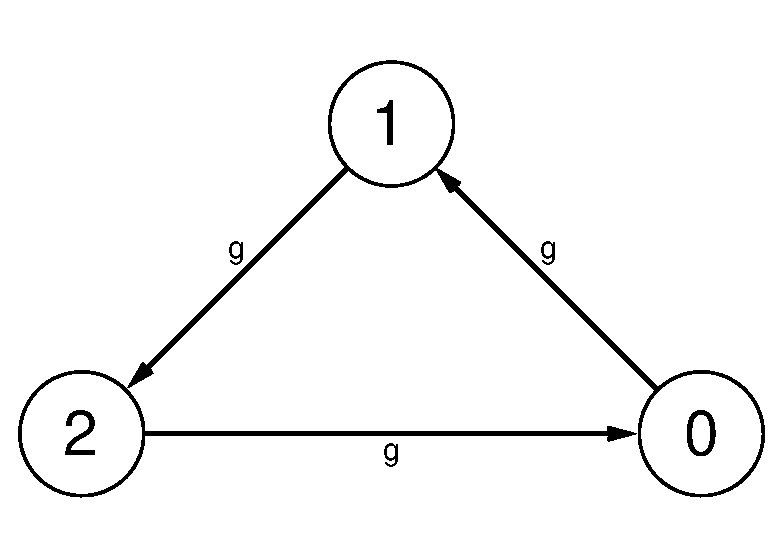
\includegraphics[width=0.35\textwidth]{fig/chap2/taxas.eps}}
\caption{\label{fig:taxas}
    Transition rates for an isolated unit.
    }
\end{center}
\end{figure}

\begin{figure}
    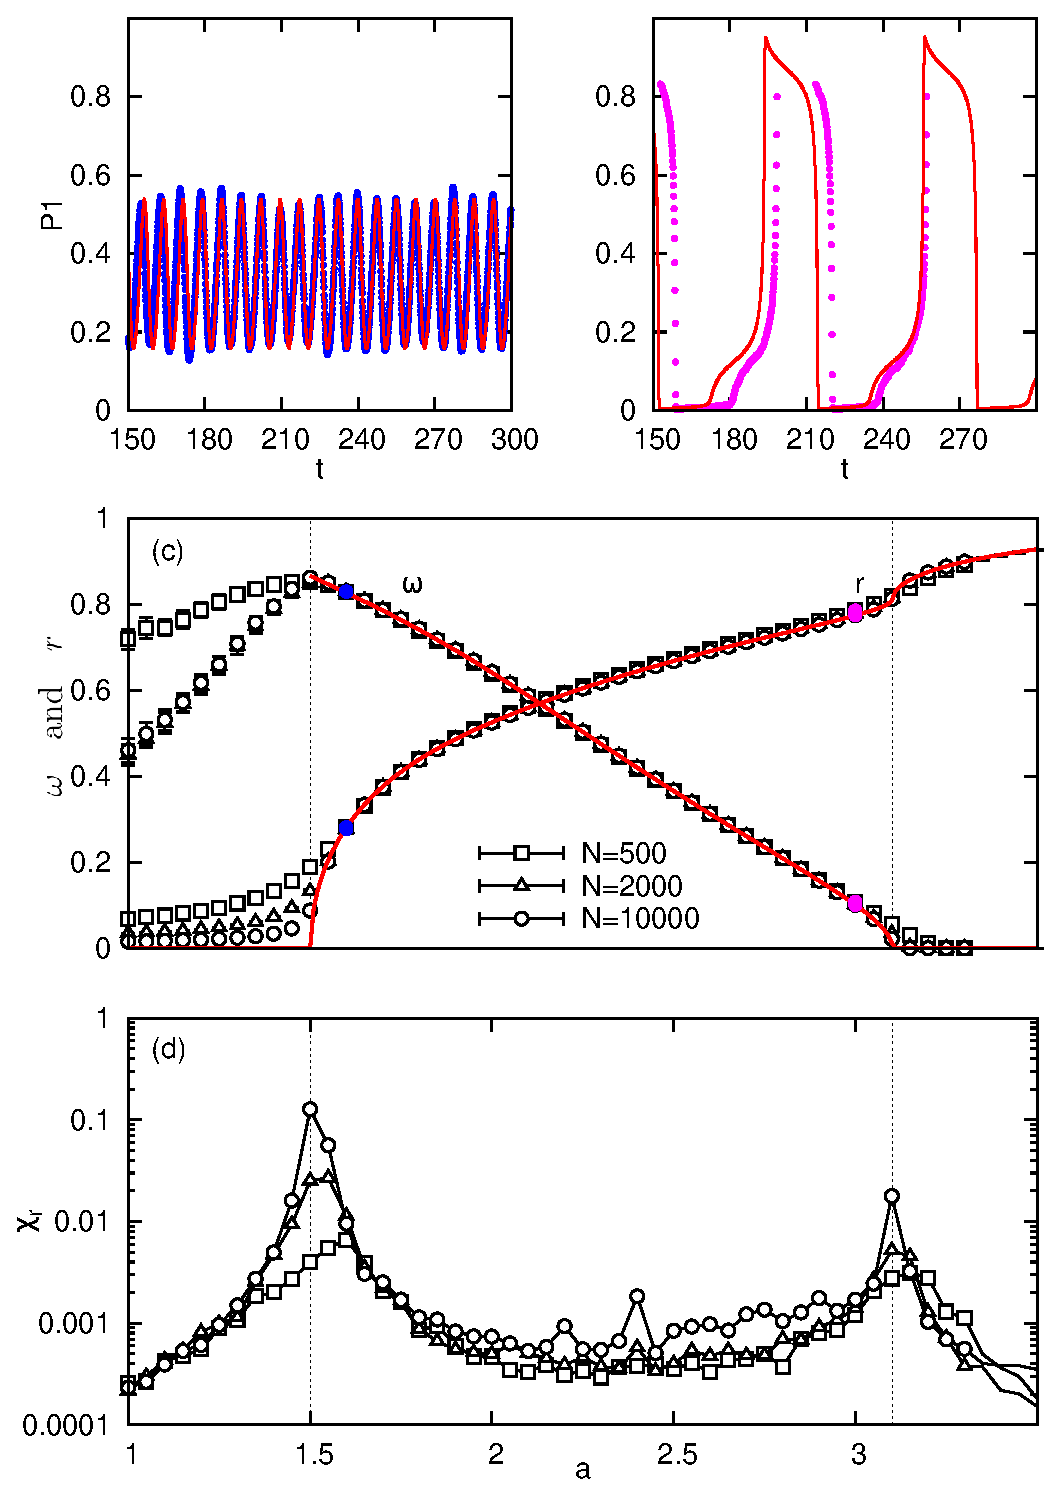
\includegraphics[height=.75\textheight]{fig/chap2/figure2.eps}
\begin{center}
\caption{\label{complete_graph} (Color online) Panels (a) and (b) show the evolution of $P_1$ for $a=1.6$ and $a=3$, respectively.
Points: simulations of a complete graph of $N$ nodes; lines: MF solution. (c) Dependence of $r$ and $\omega$ on $a$, exhibiting the two
phase transitions. (d) $\chi_r$ versus $a$, showing peaks at the transitions [system sizes as in (c)].  }
\end{center}
\end{figure}

In the WCM, the state $s^x$ at site $x$ ($x=1,\ldots,N$) can take one of three values, $s^x \in \{0,1,2\}$, corresponding to a phase
$\phi^x = 2 \pi s_x/3$.  The only allowed transitions are those from $s$ to $s+1$ (modulo 3) (see Fig.~\ref{fig:taxas}), which implies
that detailed balance is violated. If site $x$ is in state $s^x=j$, its transition rate to state $j+1$ is:

\begin{equation}
\label{eq:gj}
\gamma^x_j = g \exp \left[ a\frac {\left( n^x_{j+1} - n^x_j \right)} {n^x} \right]
\end{equation}

\noindent where $g$ is a constant, $a$ is the coupling parameter, $n^x_j$ is the number of neighbors of site $x$ in state $j$, and
$n^x$ is the number of neighbors for site $x$. Since these rates are invariant under cyclic permutation of the state indices, the model
is invariant under the group $C_3$ of discrete rotations.

Let $N_j$ be the total number of sites in state $j$, so that $N_0 +N_1 +N_2 = N$, the total number of sites. As discussed in
\cite{assis2011infinite}, the MF approximation, obtained by replacing $n^x_j/n^x$ in the argument of the exponential
of~Eq.(\ref{eq:gj}) with the corresponding state fraction, $n_j = N_j/N$, yields three non equilibrium phases, separated by two
continuous phase transitions. For small coupling ($a < a_c = 1.5$), the disordered phase, with $\textbf{n}=(1/3,1/3,1/3) \equiv
\textbf{n}_{1/3}$, is the stable stationary solution of the MF equations. ($\textbf{n}$ denotes the vector of state fractions.) For $a$
between $a_c$ and a higher value, $a^c\simeq 3.102\, 439\, 915\, 64$, there is no stable stationary solution and the MF equations admit
an oscillatory solution (a limit cycle) in which states 0, 1 and 2 periodically assume the role of the majority. As $a$ is increased
above $a_c$, the frequency $\omega$ of oscillation decreases continuously, becoming zero at $a^c$, signalling the IP transition.  For
$a> a^c$, three stationary solutions, \textbf{n}$_j$ appear, such that state $j$ represents the (permanent) majority. Thus $C_3$
symmetry is broken for $a > a^c$. (The three solutions are, naturally, related via cyclic permutation of indices in state space.) 

The WCM is characterized by a pair of order parameters. First, one has the familiar Kuramoto synchronization parameter
~\cite{Kuramoto84,Strogatz00,Wood06a},

\begin{equation}
    r \equiv \left<\left< |v| \right>_t\right>_s,
    \label{eq:r}
\end{equation}
\noindent where
\begin{equation}
    v \equiv \frac{1}{N} \sum^{N}_{x=1} e^{i\phi^x}.
    \label{eq:v}
\end{equation} 

\noindent In Eq.~(\ref{eq:r}),  $\left< \right>_t$ denotes a time average over a single realization (in the stationary state), and
$\left< \right>_s$ an average over independent realizations. Note that $r > 0$ is consistent with, but does not necessarily imply,
globally synchronized oscillation. The latter is characterized by a periodically varying phase of
$v$~\cite{Kuramoto92a,Ohta08,ShinomotoKuramoto86,Rozenblit11}.

In the MF analysis, the transition to the synchronized regime (the GO transition) is associated with a supercritical Hopf bifurcation
at $a=a_c=1.5$: the trivial fixed point $\textbf{n}_{1/3}$ loses stability at $a=a_c$, and a limit cycle encircling this point appears.
For $a \gtrsim a_c$, sustained oscillations in $n_j$ characterize synchronization among the oscillators (Fig.~\ref{complete_graph}a).
Correspondingly, $r$ grows continuously $\sim (a-a_c)^\beta$ at the transition (Fig.~\ref{complete_graph}c), with a MF exponent $\beta
= 1/2$~\cite{Wood06a}. The scaled variance

\begin{equation}
    \chi_r \equiv L^d \left[ \left< \left< |v| \right>^2_t \right>_s - r^2 \right],
    \label{eq:chir}
\end{equation}

\noindent diverges with the system size at criticality, as shown in Fig.~\ref{complete_graph}d for simulations on the complete graph
\cite{assis2011infinite}. The GO transition is associated with breaking of the continuous time-translation symmetry: the
$\textbf{n}_k(t)$, are periodic for $a\gtrsim a_c$.  Increasing $a$ above $a_c$ enhances synchronization among the oscillators, leading
to increasing oscillation amplitudes, as shown in Fig.~\ref{complete_graph}b.

Wood \textit{et al.} found that the increasing amplitude of oscillation is accompanied by a decreasing angular frequency $\omega =
2\pi/\langle \tau \rangle$, where $\langle \tau \rangle$ is the mean time between peaks in $n_k$ (Figs.~\ref{complete_graph}a-c). This
can be understood qualitatively from the exponential dependence of the transition rates of Eq.~(\ref{eq:gj}) on the neighbor fractions:
When a state is highly populated, the rate at which oscillators leave it becomes very small.  In the MF theory, when $a$ reaches the
upper critical value $a^c$, three symmetric saddle-node bifurcations occur simultaneously, and the period of the collective
oscillations diverges \cite{assis2011infinite}. Above $a^c$, there are three symmetric attractors in the system, and 3-fold rotational
($C_3$) symmetry is spontaneously broken.  As in condensation or a ferromagnetic phase transition~\cite{Huang}, freezing of the
majority state does not imply that individual oscillators freeze as well.  The transition rates of individual oscillators do decrease
with increasing $a$, but only vanish in the limit $a\to\infty$, when one of the states is fully occupied.

It is convenient to define an order parameter $\psi$ that is identically zero (in the infinite-size limit) for $a>a^c$. Assis et al.
proposed \cite{assis2011infinite},
\vspace{1em}

\begin{equation}
    \label{eq:psi}
    |\psi| \equiv \frac{1}{N}\left| \sum_{x=1}^N \left( \delta_{0,s^x} + e^{2\pi i/3}\delta_{1,s^x} + e^{-2\pi i/3}\delta_{2,s^x} \right) \gamma^x \right|
\end{equation}
\vspace{1em}

\noindent where $\delta_{ij}$ is the Kronecker delta and $\gamma^x \equiv \gamma^x_{s^x}$ is the transition rate at site $x$ (see
eq.~\ref{eq:gj}). Thus $|\psi|$ involves not only the configuration, but the rate at which the latter evolves.  On the complete graph,
$\gamma^x$ is the same for all sites $x$ in the same state $j$. Denoting this rate by $\gamma_j$, the order parameter can be written
(in MF analysis) as

\begin{equation}
    \label{eq:psiMF}
    |\psi|^2 \stackrel{MF}{=} \sum_{j=0}^2 (n_j \gamma_j - n_{j-1} \gamma_{j-1})^2 
\end{equation}

\noindent Both the disordered phase ($a< a_c$) as well as the IP phase ($a>a^c$) have stable, stationary solutions, $\textbf{n}^*$.
Since $\dot{n}_j = 0$ implies $n^*_j\gamma_j = n^*_{j-1}\gamma_{j-1}$, i.e., zero net change in the probability of state $j$, we have
$|\psi|=0$ in eq.~\ref{eq:psiMF} for both cases [a similar line of reasoning can be applied directly to Eq.~(\ref{eq:psi})].

\begin{figure}
\begin{center}
    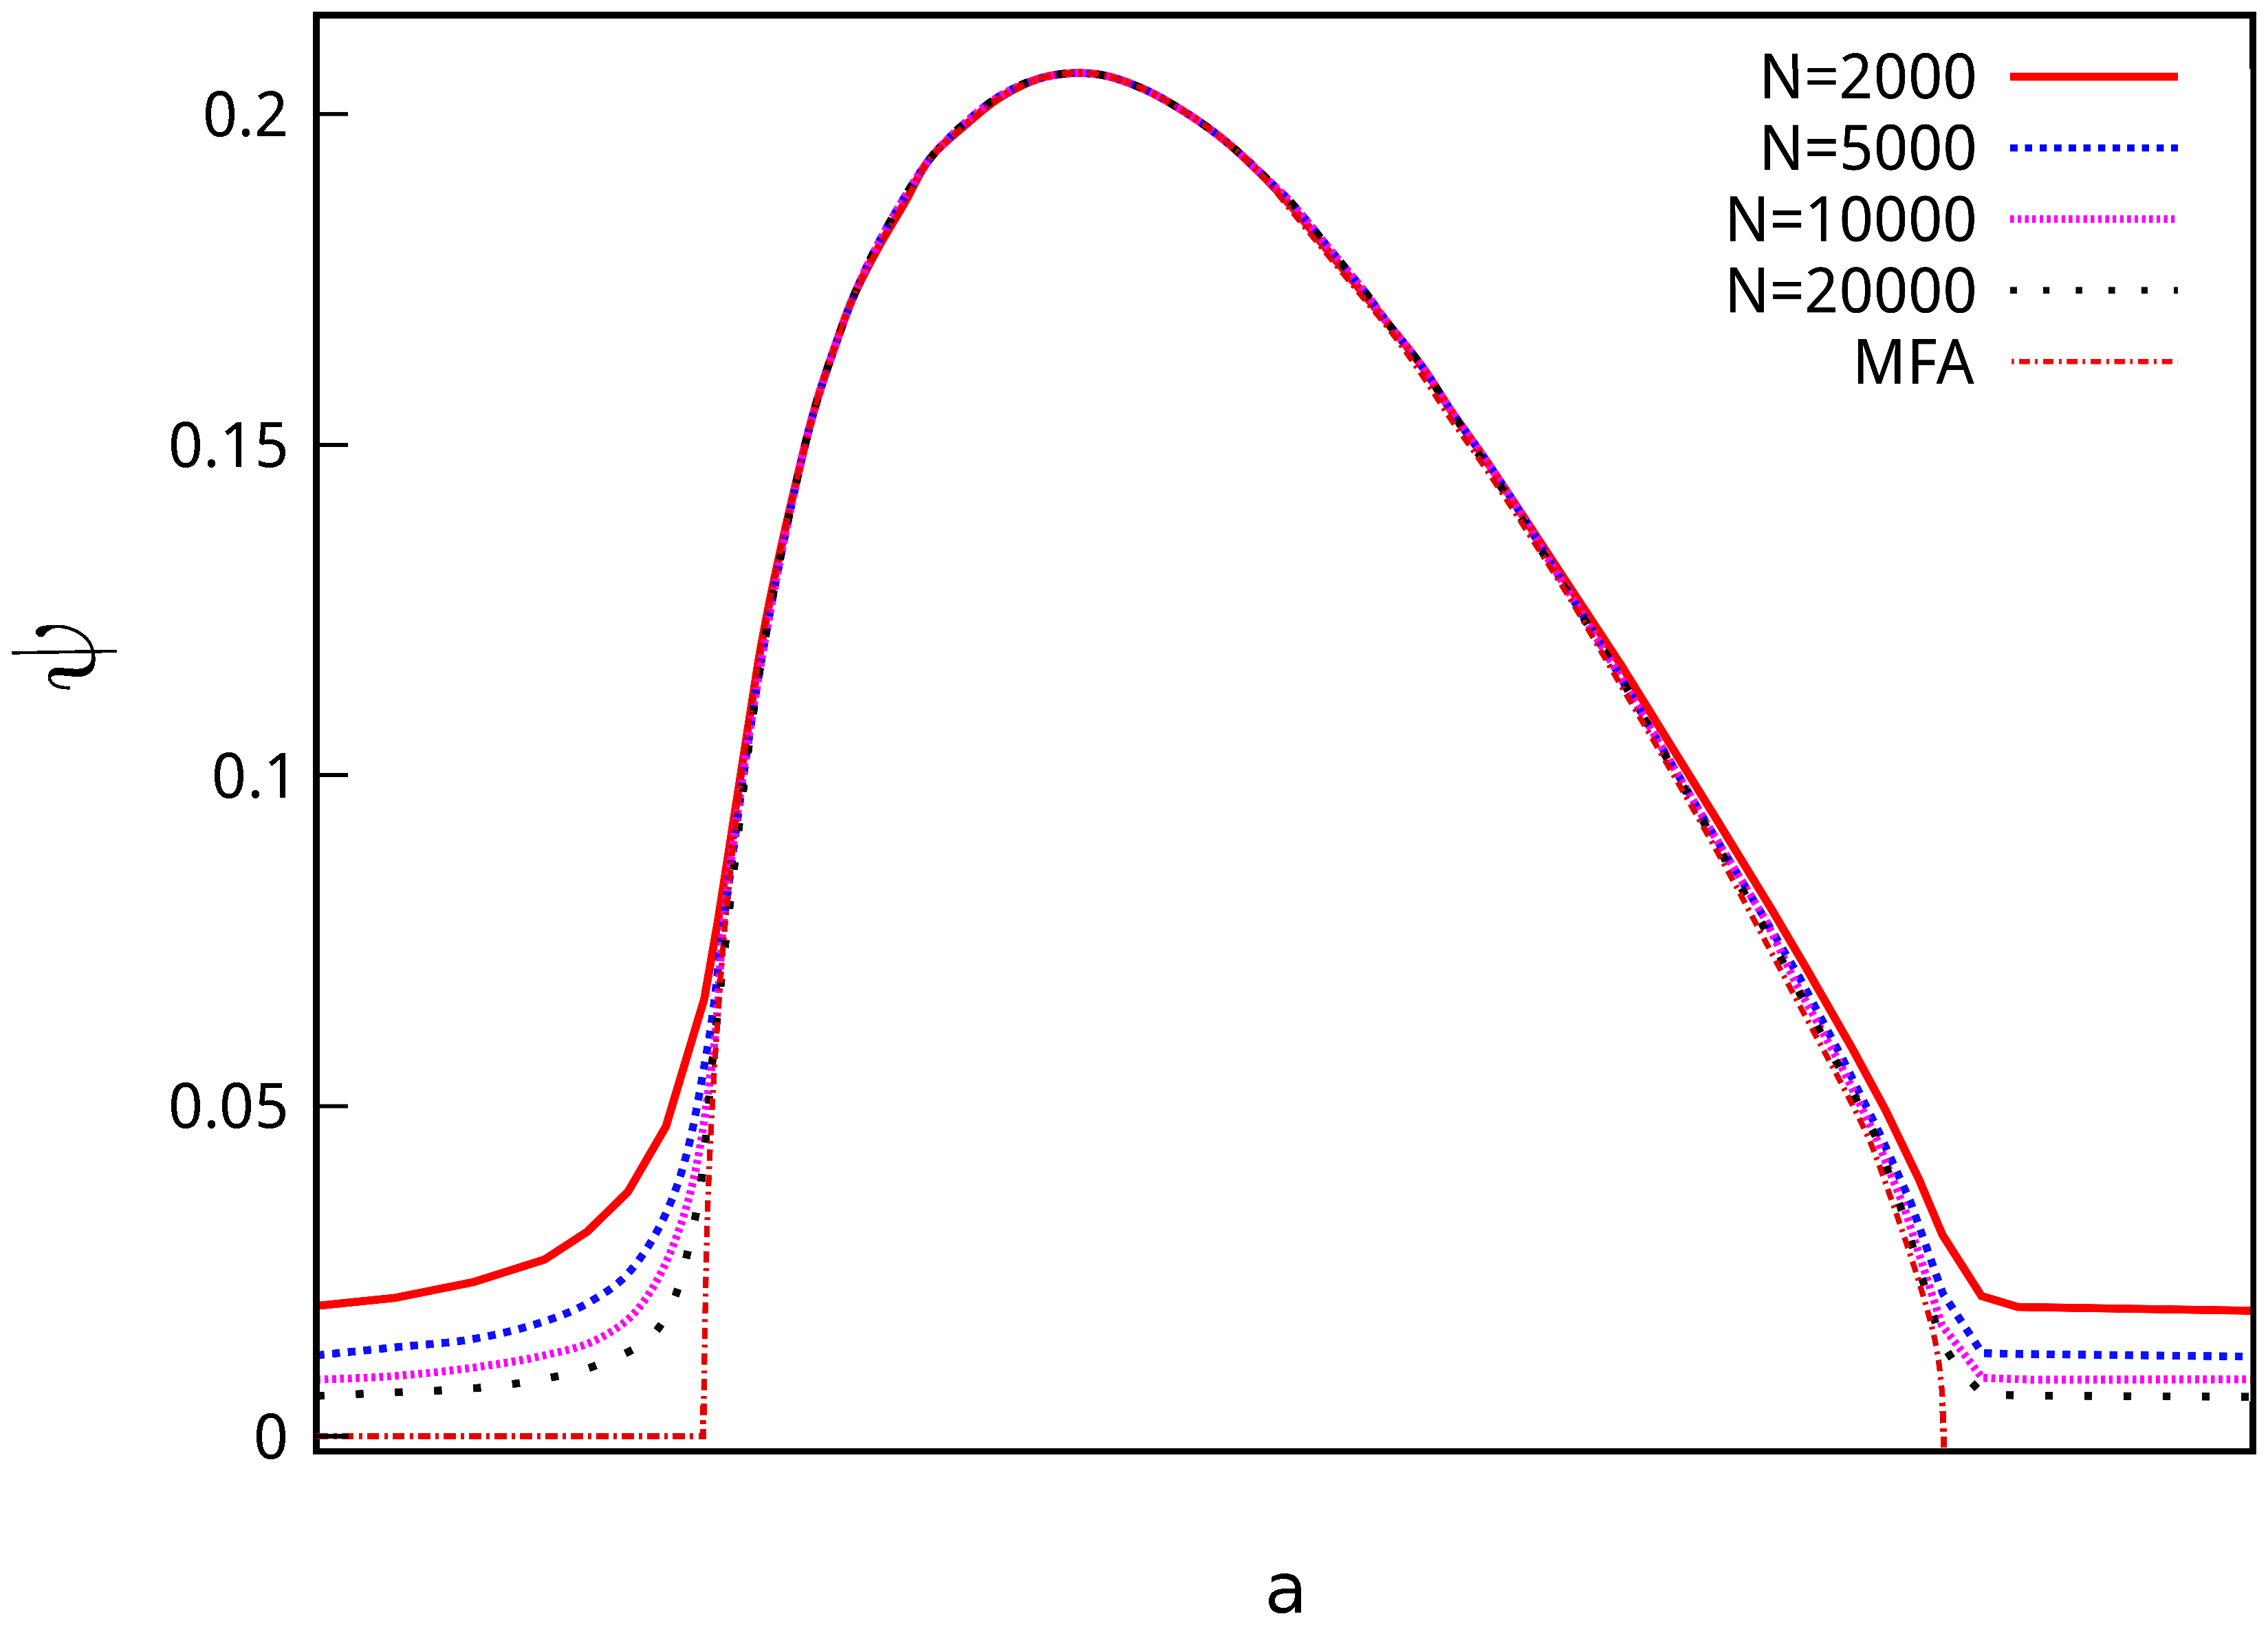
\includegraphics[width=0.7\textwidth]{fig/chap2/psivsa.eps}
    \caption{\label{fig:psi}
        (Color online) (From \cite{assis2011infinite}.) Order parameter $\langle
        |\psi| \rangle$ as a function of coupling $a$ in the MF theory and
        on the complete graph, for sizes as indicated.
    }
\end{center}
\end{figure}

Figure \ref{fig:psi} shows $\langle |\psi| \rangle$ versus $a$ in MF theory, and on the complete graph (the latter via numerically
exact solution of the master equation), confirming that $|\psi|$ functions as an order parameter to detect both the GO and IP phase
transitions. The MF critical behavior is $\langle |\psi| \rangle \sim (a- a_c)^{1/2} $ for $a \searrow a_c$ and $\langle |\psi| \rangle
\sim (a^c - a)^{1/2}$ for $a \nearrow a^c$.  On the complete graph, the order parameter decays with system size as $\langle |\psi|
\rangle \sim N^{-1/4}$ at $a=a_c$ and as $N^{-0.4203(3)}$ at $a=a^c$. The first result is typical of MF scaling with system size at a
continuous phase transition, as argued in \cite{assis2011infinite}.

The results for the IP transition in MF and on a complete graph are in sharp contrast to what is found on finite-dimensional lattices.
The \textit{absence} of such a transition was verified numerically on hyper cubic lattices in dimensions $d \leq 4$ in
\cite{assis2011infinite}. This reference also provides a quantitative argument showing that on finite-dimensional lattices, a $j$-state
majority cannot persist indefinitely: it is always susceptible to change via nucleation of a cluster of state $j+1$. The authors of
\cite{assis2011infinite} conjectured that the IP transition would occur on structures in which a site interacts with a nonzero fraction
of all other sites (as the system size tends to infinity). In the following sections we test this conjecture on two structures, regular
rings with extended interactions, and small-world networks.

\section{\label{regularrings} The WCM on regular rings }


A \textit{regular ring} is constructed starting from a graph of $N$ nodes arranged in circular fashion. Considering one node at a time in
a clockwise manner, we connect it to its $K$ nearest neighbors in the clockwise direction; an example of such a structure is shown in
Fig.~\ref{fig:ring}. We define the \textit{connectivity} of a regular ring graph by $\alpha \equiv K/N$, such that $\alpha=1/N$ signifies
a one-dimensional chain while $\alpha=0.5$ represents a complete graph. Thus, one can interpolate from the one-dimensional to an
infinite-dimensional hyper cubic lattice (complete graph) varying $\alpha$ over the interval $\left( 0, \frac{1}{2} \right]$.  It is
known that the WCM on hyper cubic lattices of dimensions 1 and 2 cannot sustain ordered phases \cite{Wood06a, assis2011infinite}. Since
$\alpha=0.5$ represents the complete graph, there must be at least one threshold $\alpha=\alpha^*$ above which one or both phase
transitions (GO and IP) occur, varying $a$.

Different from hyper cubic lattices, in which coupling is local, for $\alpha > 0$ the coupling on ring graphs is nonlocal.  The manner
in which the interaction range scales as $N\to\infty$ can be chosen in different ways; the simplest, which we consider here, is to fix
$\alpha$ so that $K \propto N$ (More precisely,  $K=\lceil\alpha N\rceil$ where $\lceil x \rceil$ denotes the smallest integer larger
than $x$).  It is reasonable to expect that phase transitions occur for any fixed $\alpha > 0$, since the interaction range $K$ then
tends to infinity with $N$. 

\begin{figure}[b]
\begin{center}
    \fbox{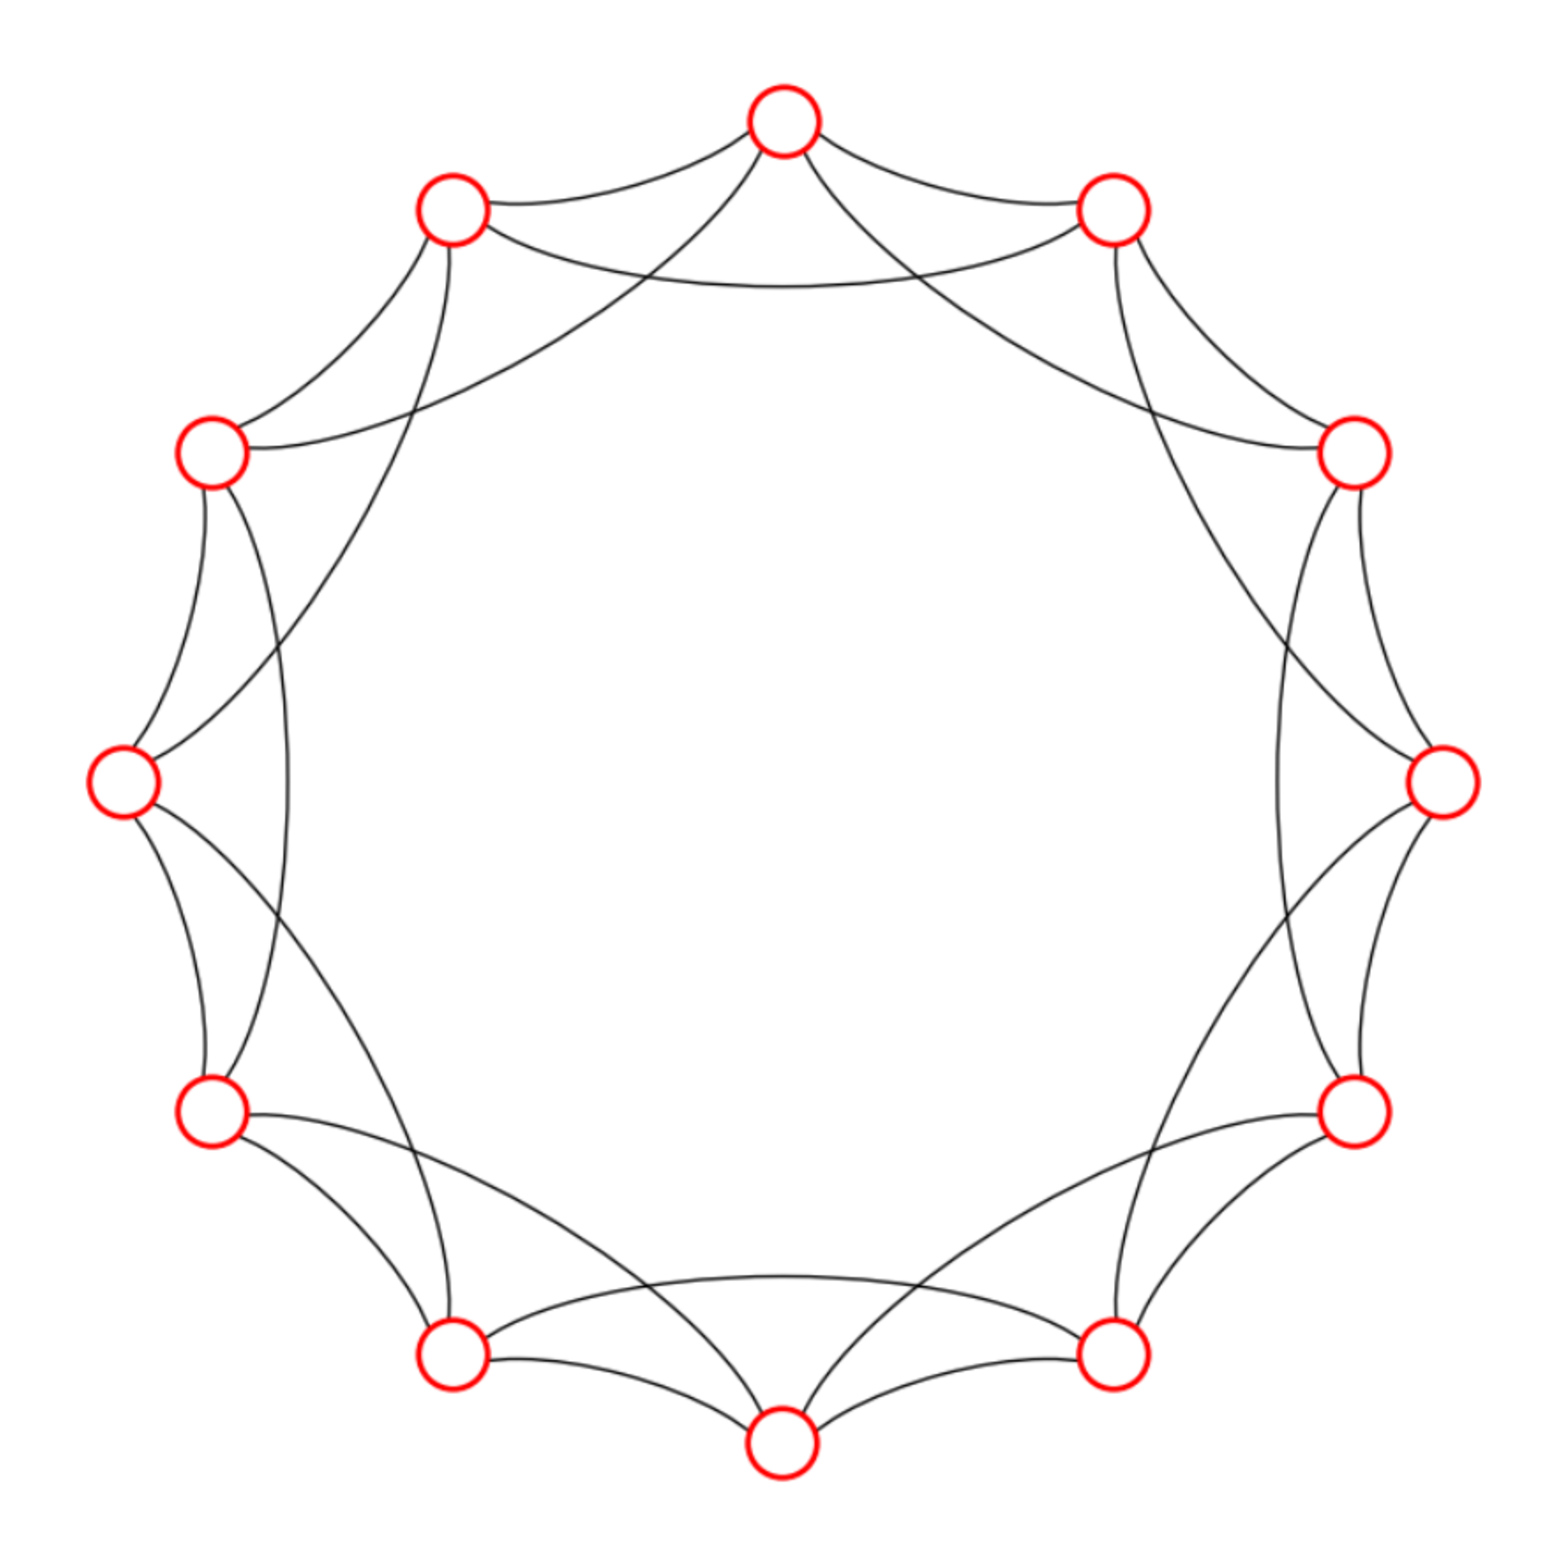
\includegraphics[width=0.40\textwidth]{fig/chap2/ring.eps}}
\caption{\label{fig:ring}
    A regular ring is an undirected graph with $N$ nodes arranged in circular
    fashion, with each connected to its $K$ nearest neighbors in each direction.
    Here we show an example with $N=12$ and $K=2$.
    }
\end{center}
\end{figure}

\begin{figure}[t]
\begin{center}
    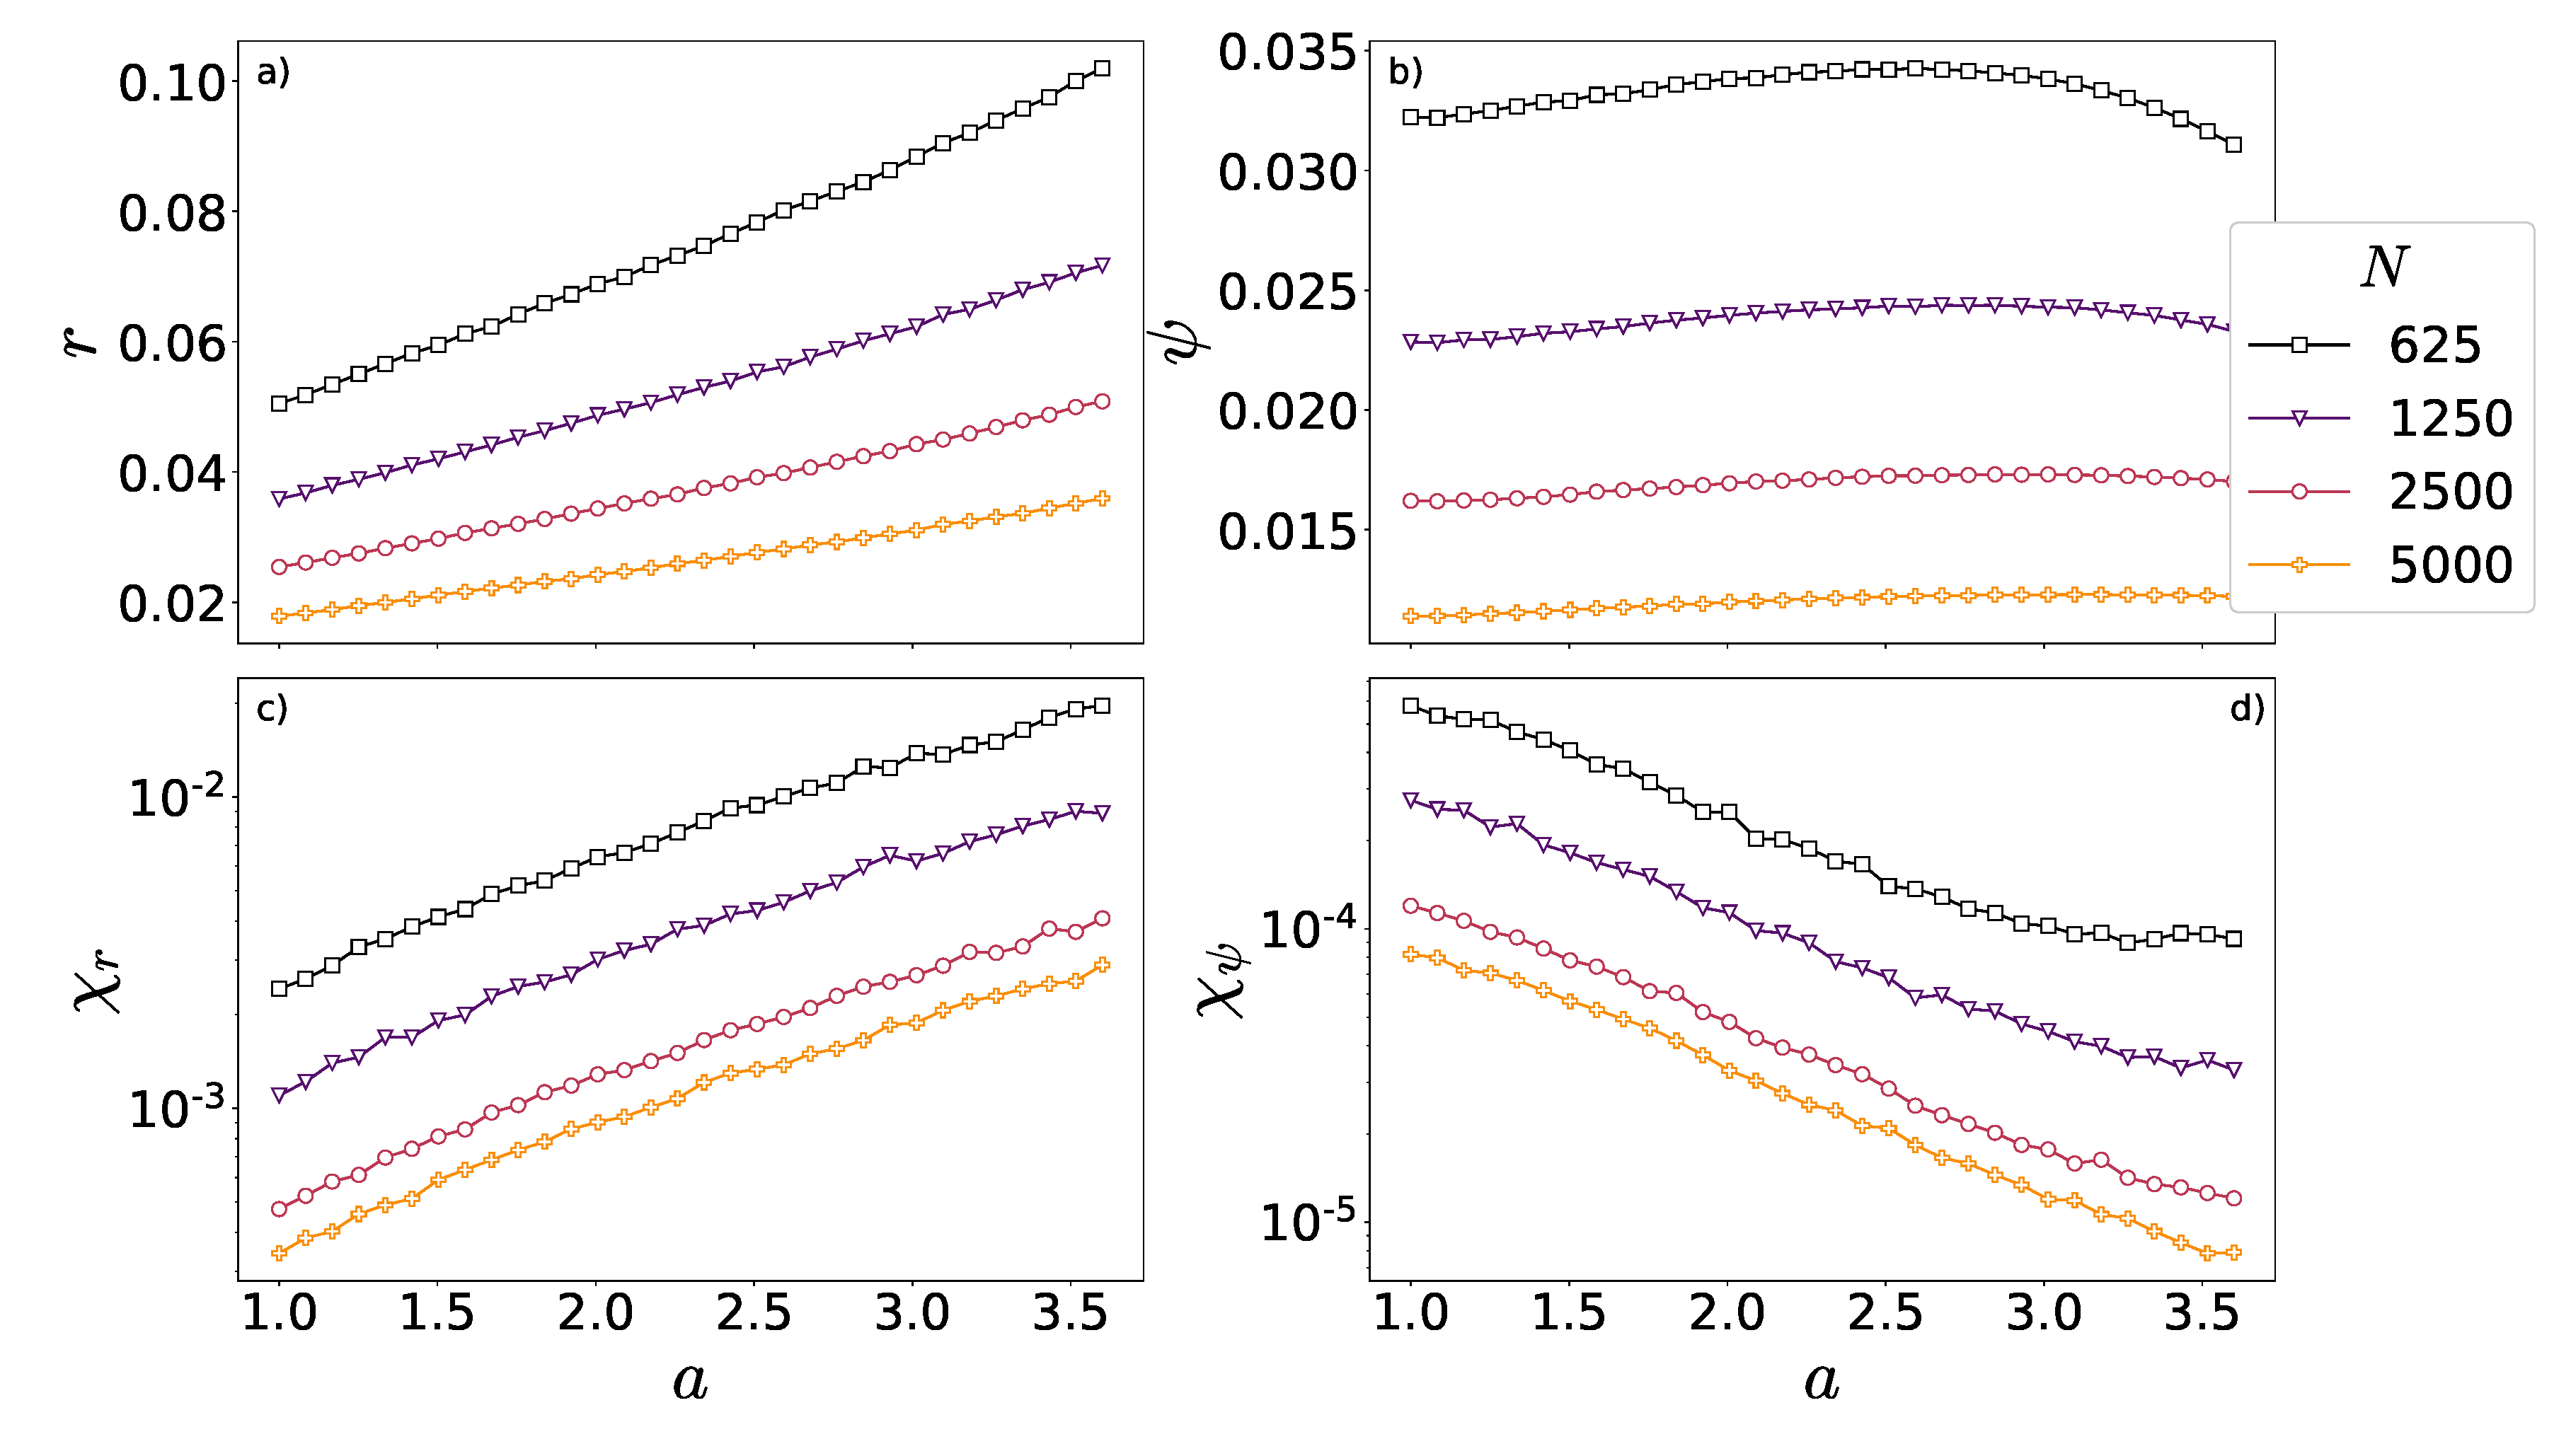
\includegraphics[width=0.9\textwidth]{fig/chap2/chi_curves_1D.eps}
\caption{\label{fig:chi_curves_1D}
    (Color online) Order parameters and their scaled variances for
    one-dimensional rings ($K=1$). Both the order parameters and their
    respective variances decrease as the system size is increased, with $r
    \approx \psi \approx 0$ across a wide range of coupling strengths. Points
    represent an average over 3000 independent realizations with random initial
    configurations. For the 1D chain, the same behavior is observed regardless
    of initial configuration.
    }
\end{center}
\end{figure}

\begin{figure}[t]
\begin{center}
    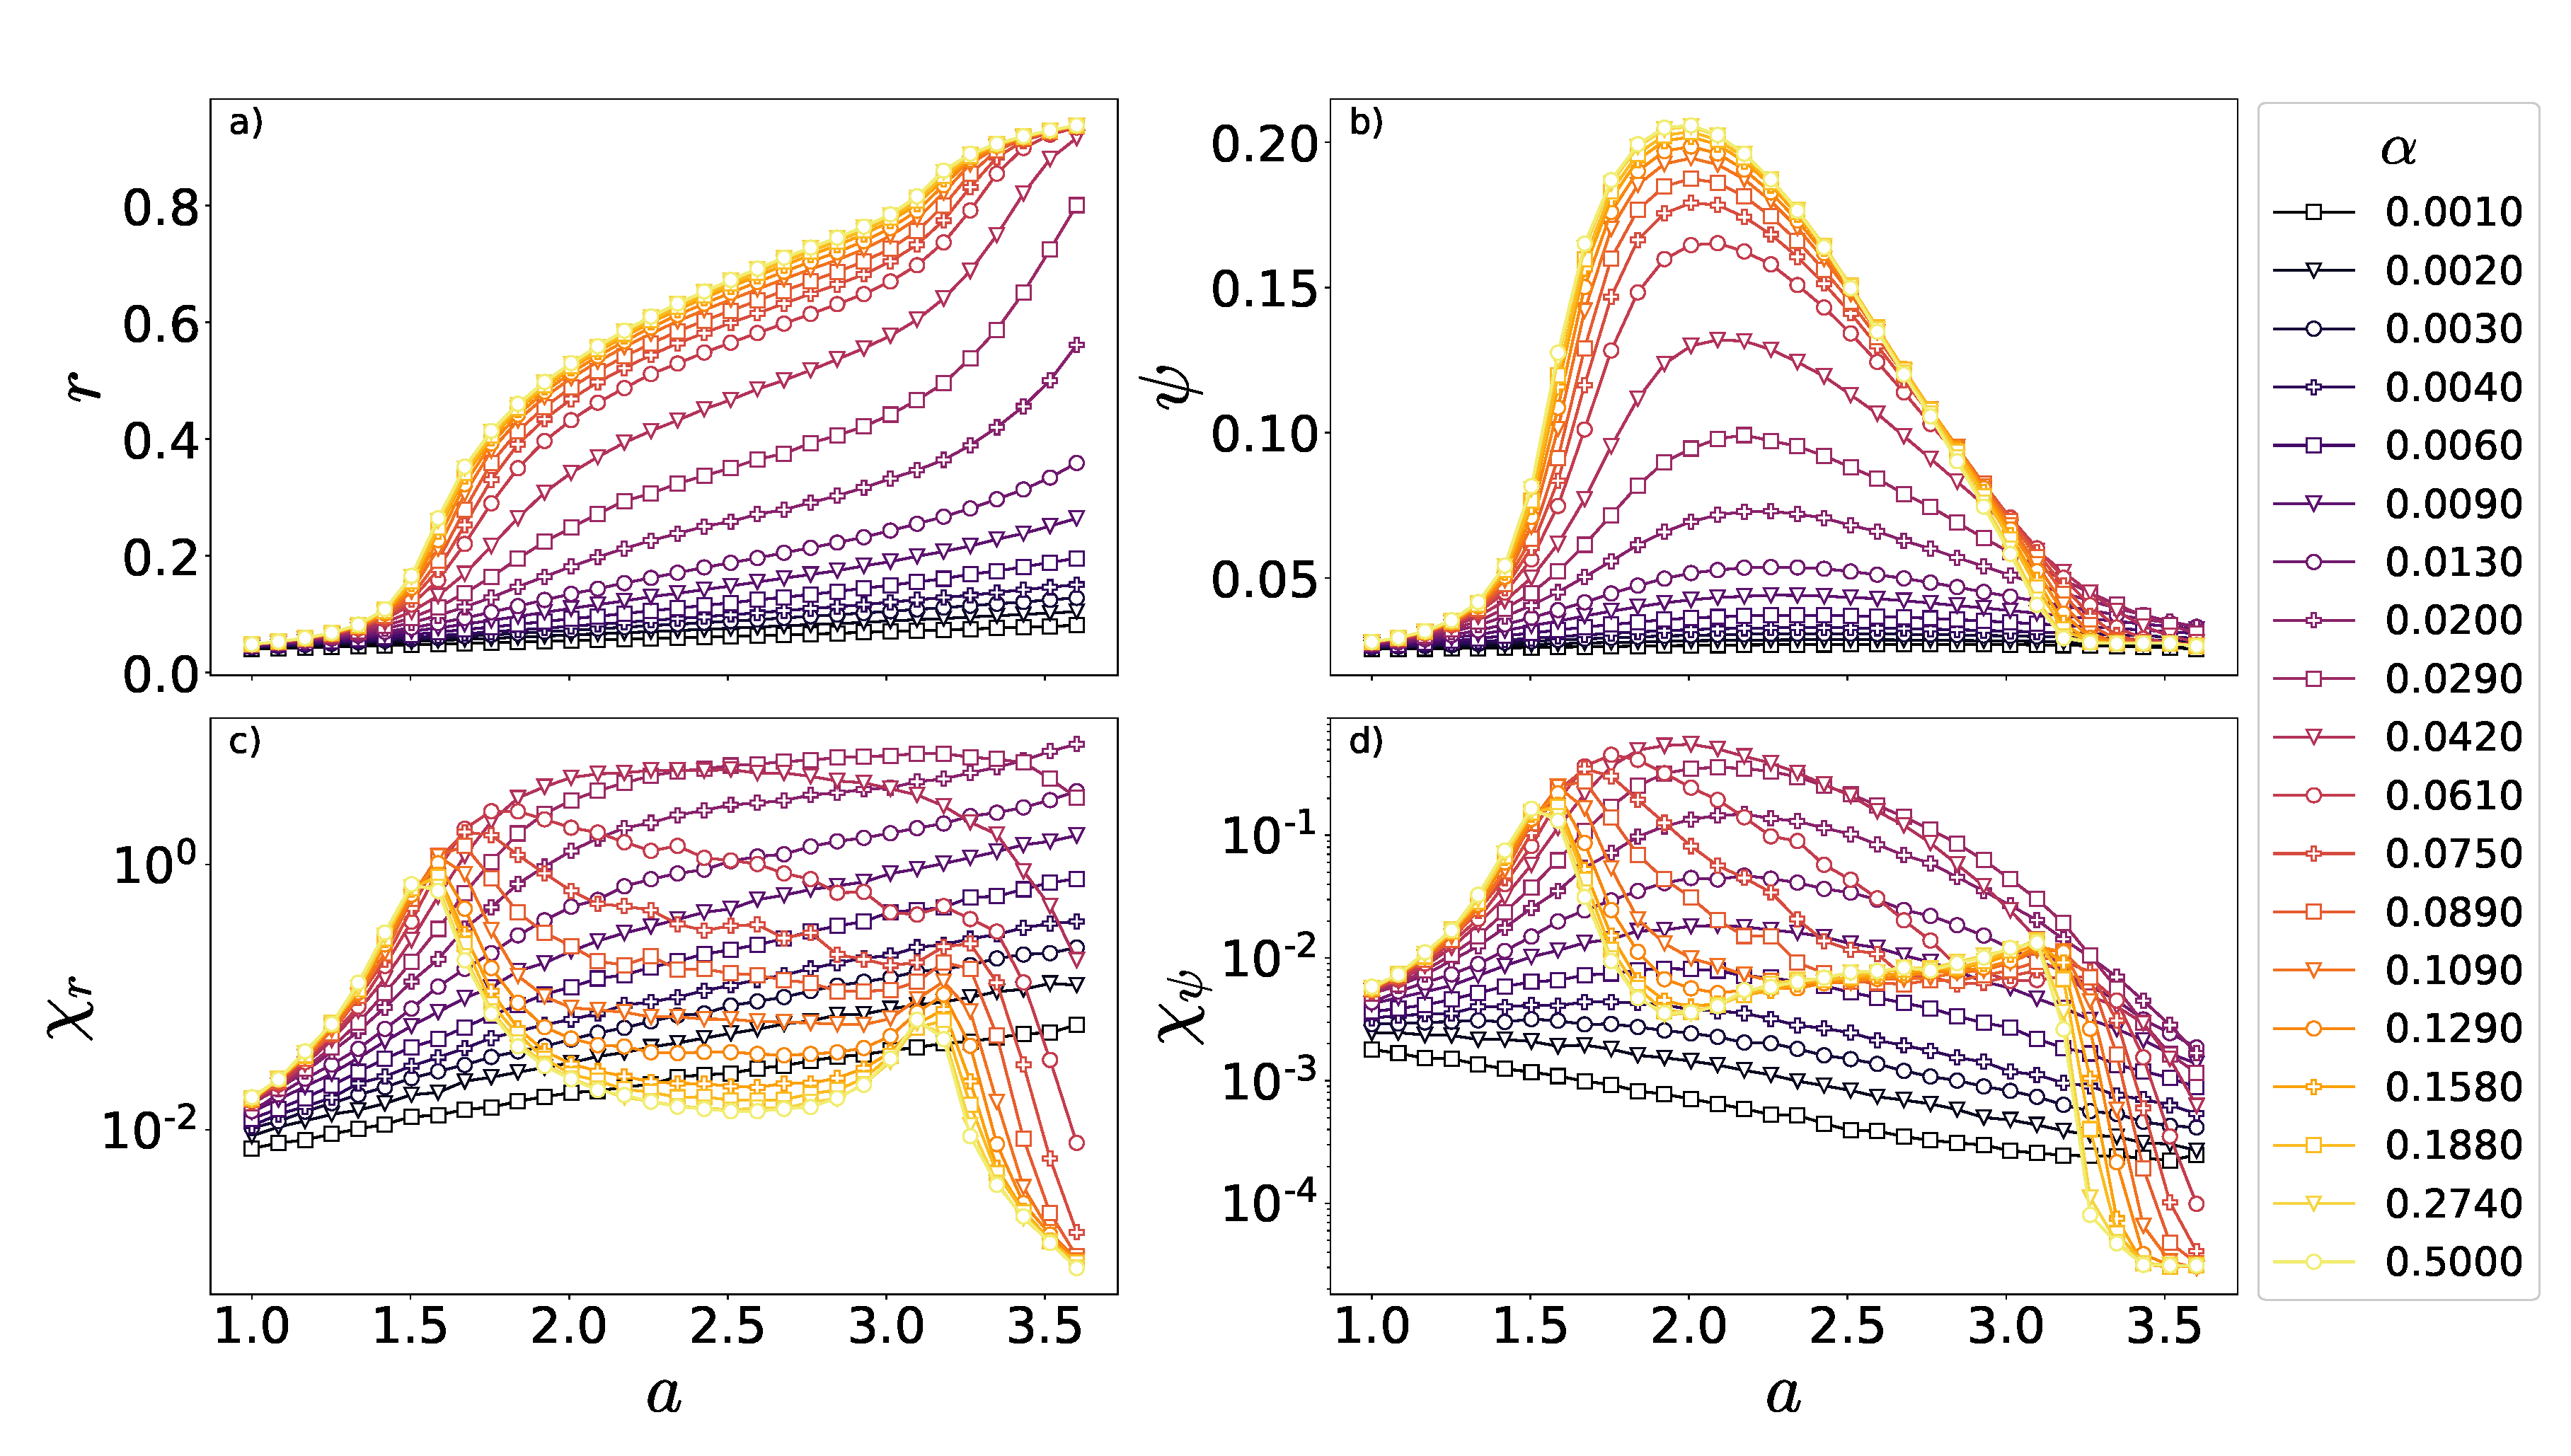
\includegraphics[width=0.95\textwidth]{fig/chap2/chi_curves_uniformic.eps}
    \caption{\label{fig:chicurves}
    (Color online) Order parameters and scaled variances for regular rings of
    size $N=1000$ and various values of the connectivity $\alpha$.  Points
    represent an average over 4000 independent realizations with uniform initial
    configurations.
    }
\end{center}
\end{figure}

\subsection{Scaling behavior: phase boundary}

The dynamics as $N$ increases can be studied by defining the scaled variances of the order parameters. These quantities are expected to
diverge in the thermodynamic limit when the system undergoes a continuous phase transition \cite{plischke1994equilibrium}.  The scaled
variances of order parameters $r$ and $\psi$ can be defined through equations \ref{eq:v} and \ref{eq:psi} as:

\begin{align}
    \chi_r &= \chirdef \notag , \\
    \chi_\psi &= \chipsidef,
\end{align}

\noindent where $\left<\right>_t$ and $\left<\right>_s$ are averages over time and over independent realizations, respectively.

In simulations, the system is allowed to relax to a steady state, starting from its initial configuration.  Once the steady state has
been attained, the order parameters are averaged over the remainder of the evolution. As we will see, the choice of initial condition
is important for some values of the interaction range $K$; we will focus on two different setups: \textit{random} initial
configurations, in which the initial phase of each oscillator is chosen uniformly and independently among the three possible values in
$\{ 0, 2\pi/3, 4\pi/3 \}$, and a \textit{uniform} initial condition, in which $\phi_i = 0, \; \forall i$.

In the following we describe results for uniform initial conditions. In Fig.~\ref{fig:chi_curves_1D} we plot the order parameters and
their associated variances for $K=1$ (i.e.,  $\alpha=1/N$). Both quantities are shown to decrease with system size (for the 1D case in
particular this behavior is the same regardless of initial configuration), indicating the absence of phase transitions. In
Fig.~\ref{fig:chicurves}, the same quantities are shown for regular rings with $N=1000$ and various $\alpha$ values.  As expected, the
order parameters and their variances approach the complete-graph limit as $\alpha$ nears the value $1/2$.  Denoting by $\alpha^*$ the
value associated with a change from one to two maxima in $\chi_{\psi}$, we identify $\alpha^* \approx 0.06$ for $N=1000$ in
Fig.~\ref{fig:chicurves}.  Performing similar analyses for different system sizes we obtain $\alpha^*$ as a function of $N$.  To infer
the scaling behavior, we define $\lambda \equiv N^{-1}$ and look at the $\alpha^*$ versus $\sqrt{\lambda}$ curve near $\lambda=0$. The
resulting data, shown in Fig.~\ref{fig:alphasplit}, suggest that $\alpha^*$ tends to zero as $N\to\infty$. This supports the conjecture
stated previously that in this limit, and for any fixed $\alpha>0$, the WCM on a regular ring lattice exhibits both GO and IP phase
transitions.

\begin{figure}
\begin{center}
    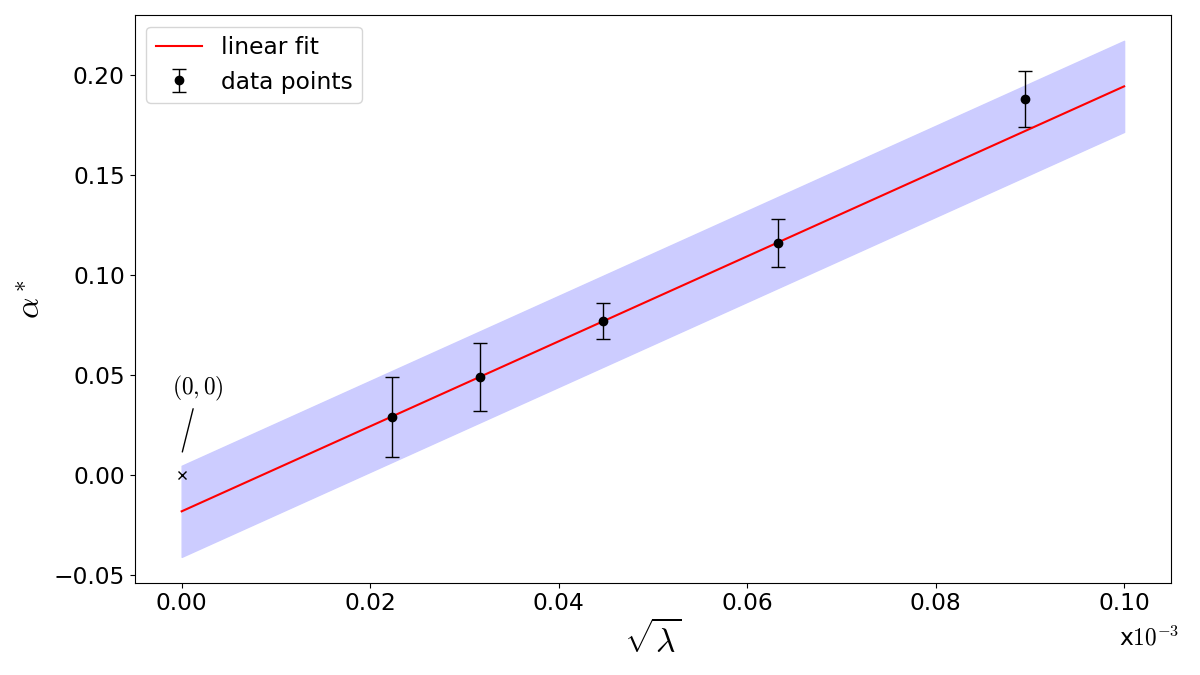
\includegraphics[width=0.9\textwidth]{fig/chap2/alphasplit.png}
    \caption{\label{fig:alphasplit} Plot of $\alpha^*$ versus $\sqrt{\lambda}$. Starting from uniform initial configurations, $\alpha >
        \alpha^*$ means $\chi_{\psi}$ and $\chi_r$ exhibit two maxima, whereas for $\alpha < \alpha^*$ only a single broad maximum is
        observed. Full circles represent data obtained from simulations and solid curve is a linear fit with equation
        $y=-0.01837+2.1271x$. The band around the fitted curve represent the uncertainty associated with the linear intercept.}
\end{center}
\end{figure}

\subsection{Scaling behavior: order parameter}

To better understand the scaling behavior we look at the order parameters as $N \to \infty$ with fixed $\alpha$. If both $r$ and $\psi$
tend to zero, there is no global synchronization. Both order parameters tending to positive values indicates the presence of global or
intermittent synchronization among large populations of oscillators, while $\psi \to 0$ with $r \sim 1$ defines an infinite-period
phase.

\begin{figure}
\begin{center}
    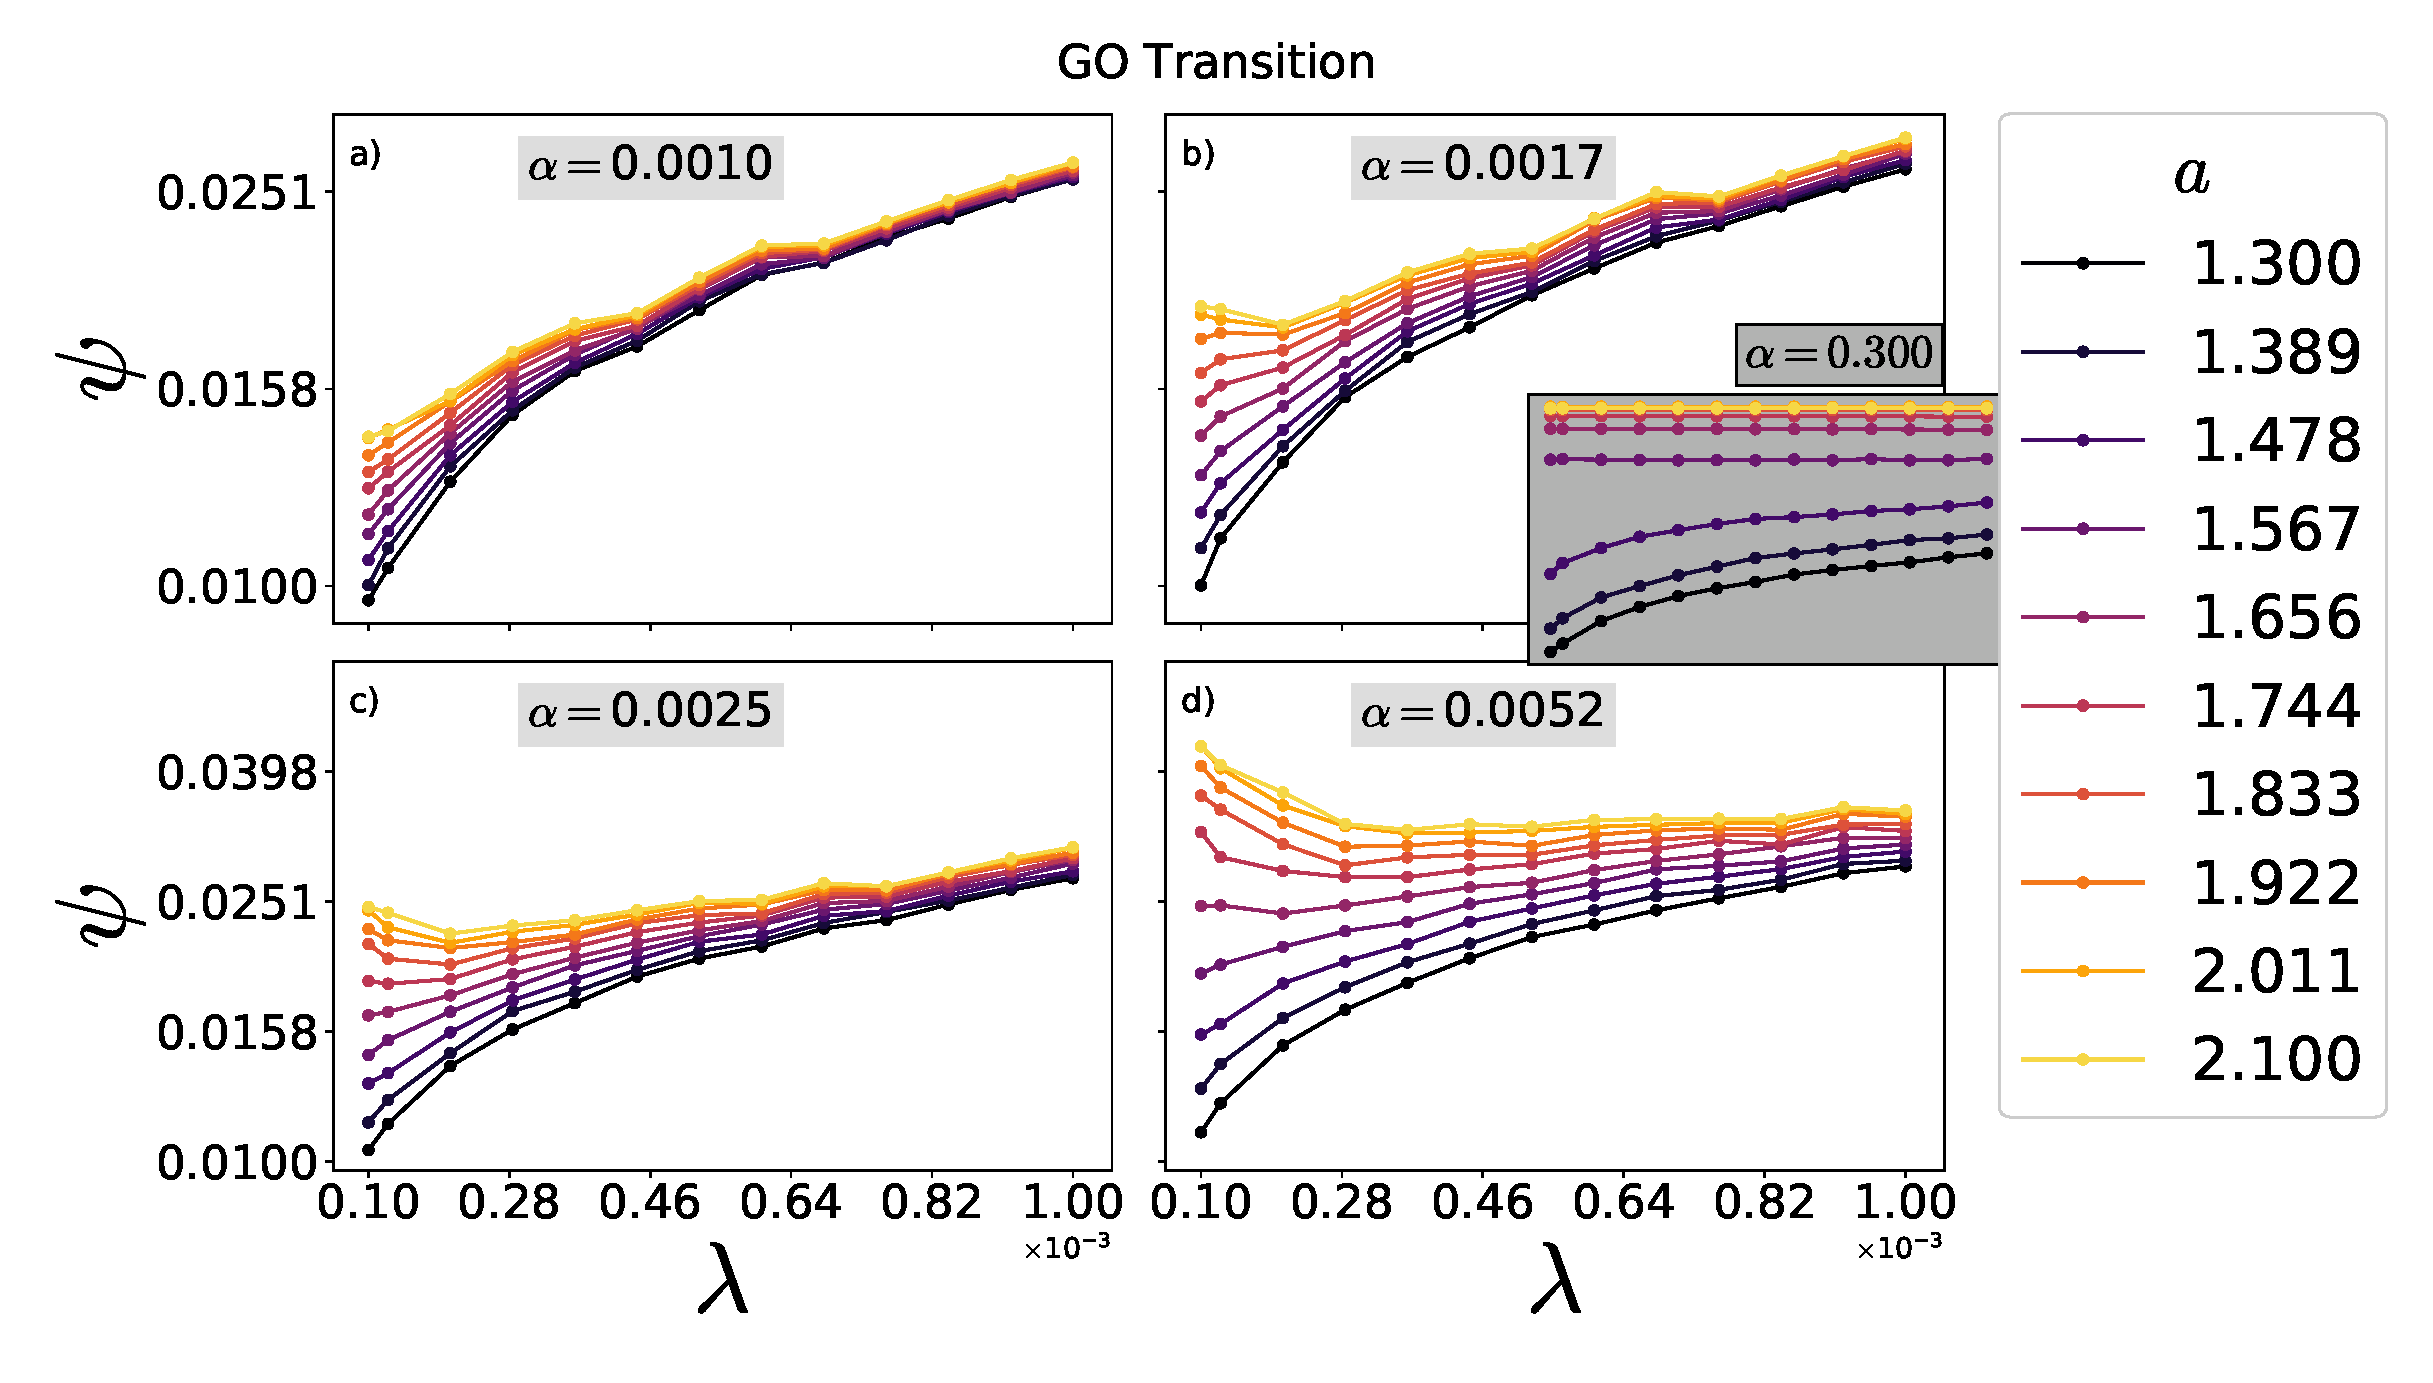
\includegraphics[width=0.85\linewidth]{fig/chap2/opsplit-psi-got.eps}
    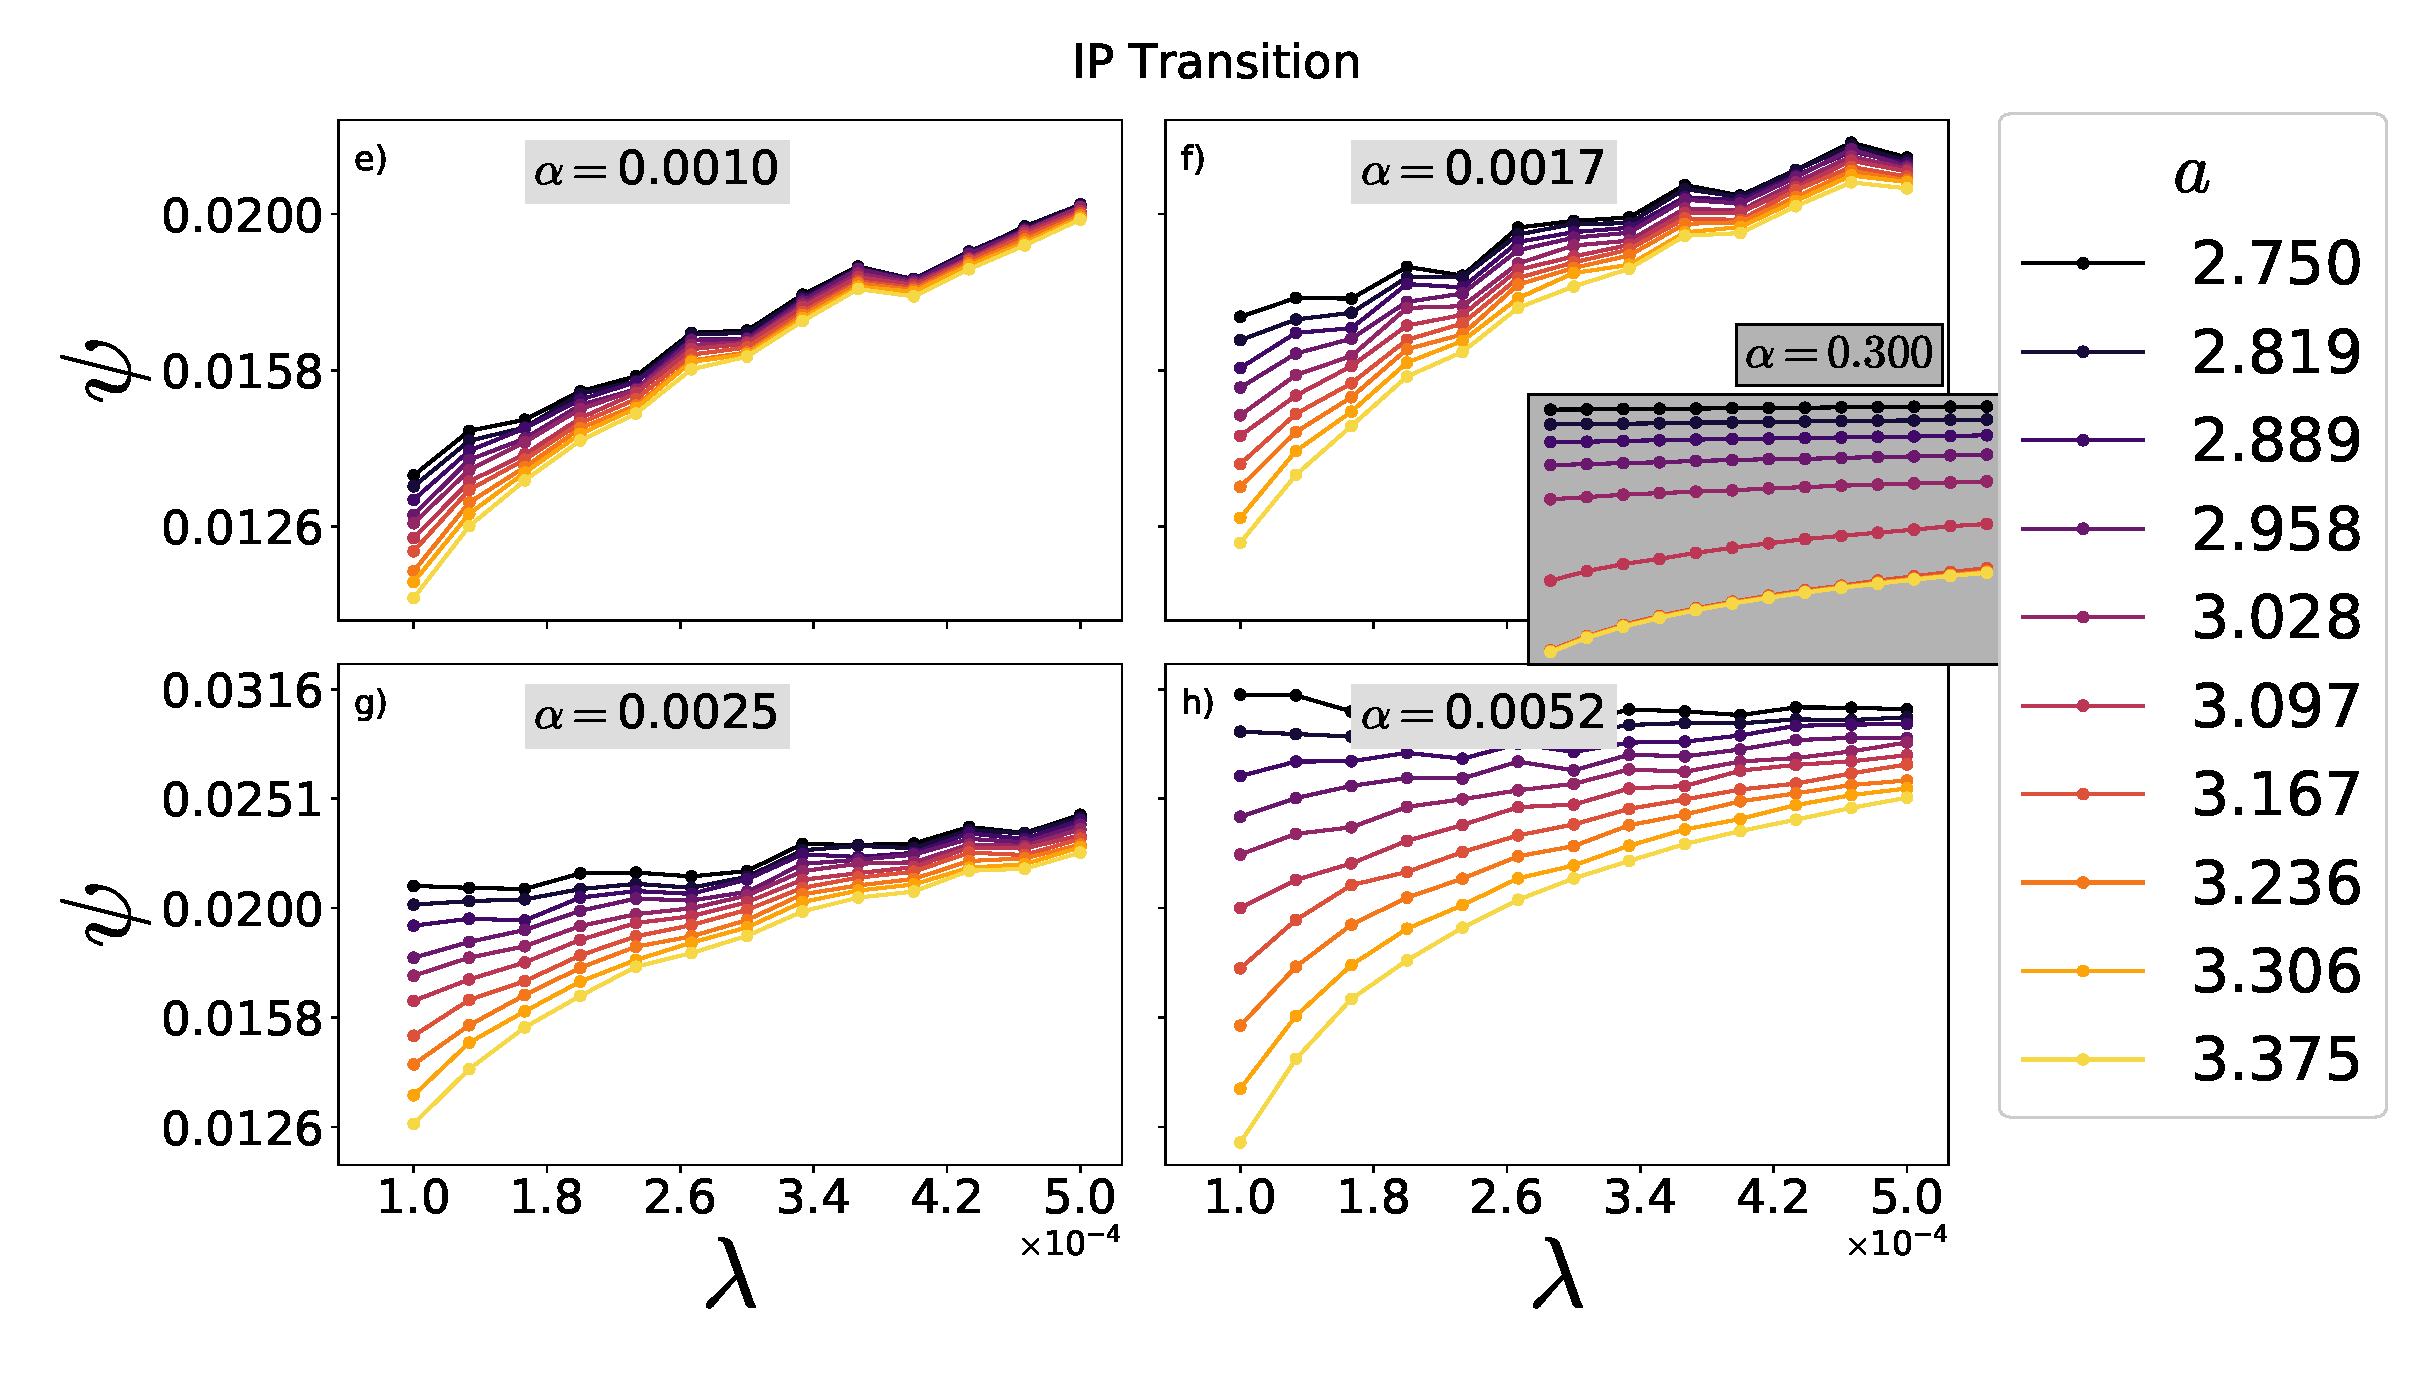
\includegraphics[width=0.85\linewidth]{fig/chap2/opsplit-psi-ipt.eps}
\end{center}
\caption{\label{fig:opsplit} (Color online) Order parameter $\psi$ versus inverse system size $\lambda$ for various values of $\alpha$,
    and coupling strengths $a$ in the vicinity of the GO and IP phase transitions. The insets in \textbf{b} and \textbf{f} show the
    behavior for $\alpha=0.3$, approaching the complete graph, with GO and IP transitions near $a_c=1.5$ and $a^c\approx3.1$
    respectively.  Each point represents an average over 400 independent realizations.  The oscillatory behavior seen in some panels is
due to the reduction in average path lengths caused by the introduction of new neighbors as the system size increases at fixed
$\alpha$, and the fact that $K$ must be an integer (see Appendix \ref{appendix:LC}).}
\end{figure}

In this context it is useful to plot the order parameter versus $\lambda\equiv1/N$. An upward (downward) curvature as $\lambda \to 0$
signals a nonzero (zero) value of the order parameter. In Fig.~\ref{fig:opsplit}, such plots are shown for selected values of $\alpha$
\footnote{{See full animations of Fig.~\ref{fig:opsplit}:
\href{https://youtu.be/pPQbc0eiv_4}{GO transition}},
\href{https://youtu.be/_qfNzoBpRO4}{IP transition}}
and system sizes up to $N=10^4$.  In panel b) we see evidence of the GO transition for the value $\alpha=0.0017$ in the form of an
inversion in curvatures for lines of constant coupling strength, which happens at $a_c \approx 2$.  The inset in this same panel shows
that for large $\alpha$ there is a clear split near the complete graph value $a_c=1.5$.  In the case of the IP transition we observe
that there is no upward curvature at any point, but rather a sharp increase in density of the lines of constant $a$ for higher values
of $\alpha$, as seen in the bottom inset of Fig.~\ref{fig:opsplit} where the lines $a=3.375$ and $a=3.306$ have collapsed to the same
point near the origin.

\begin{figure}
\begin{center}
    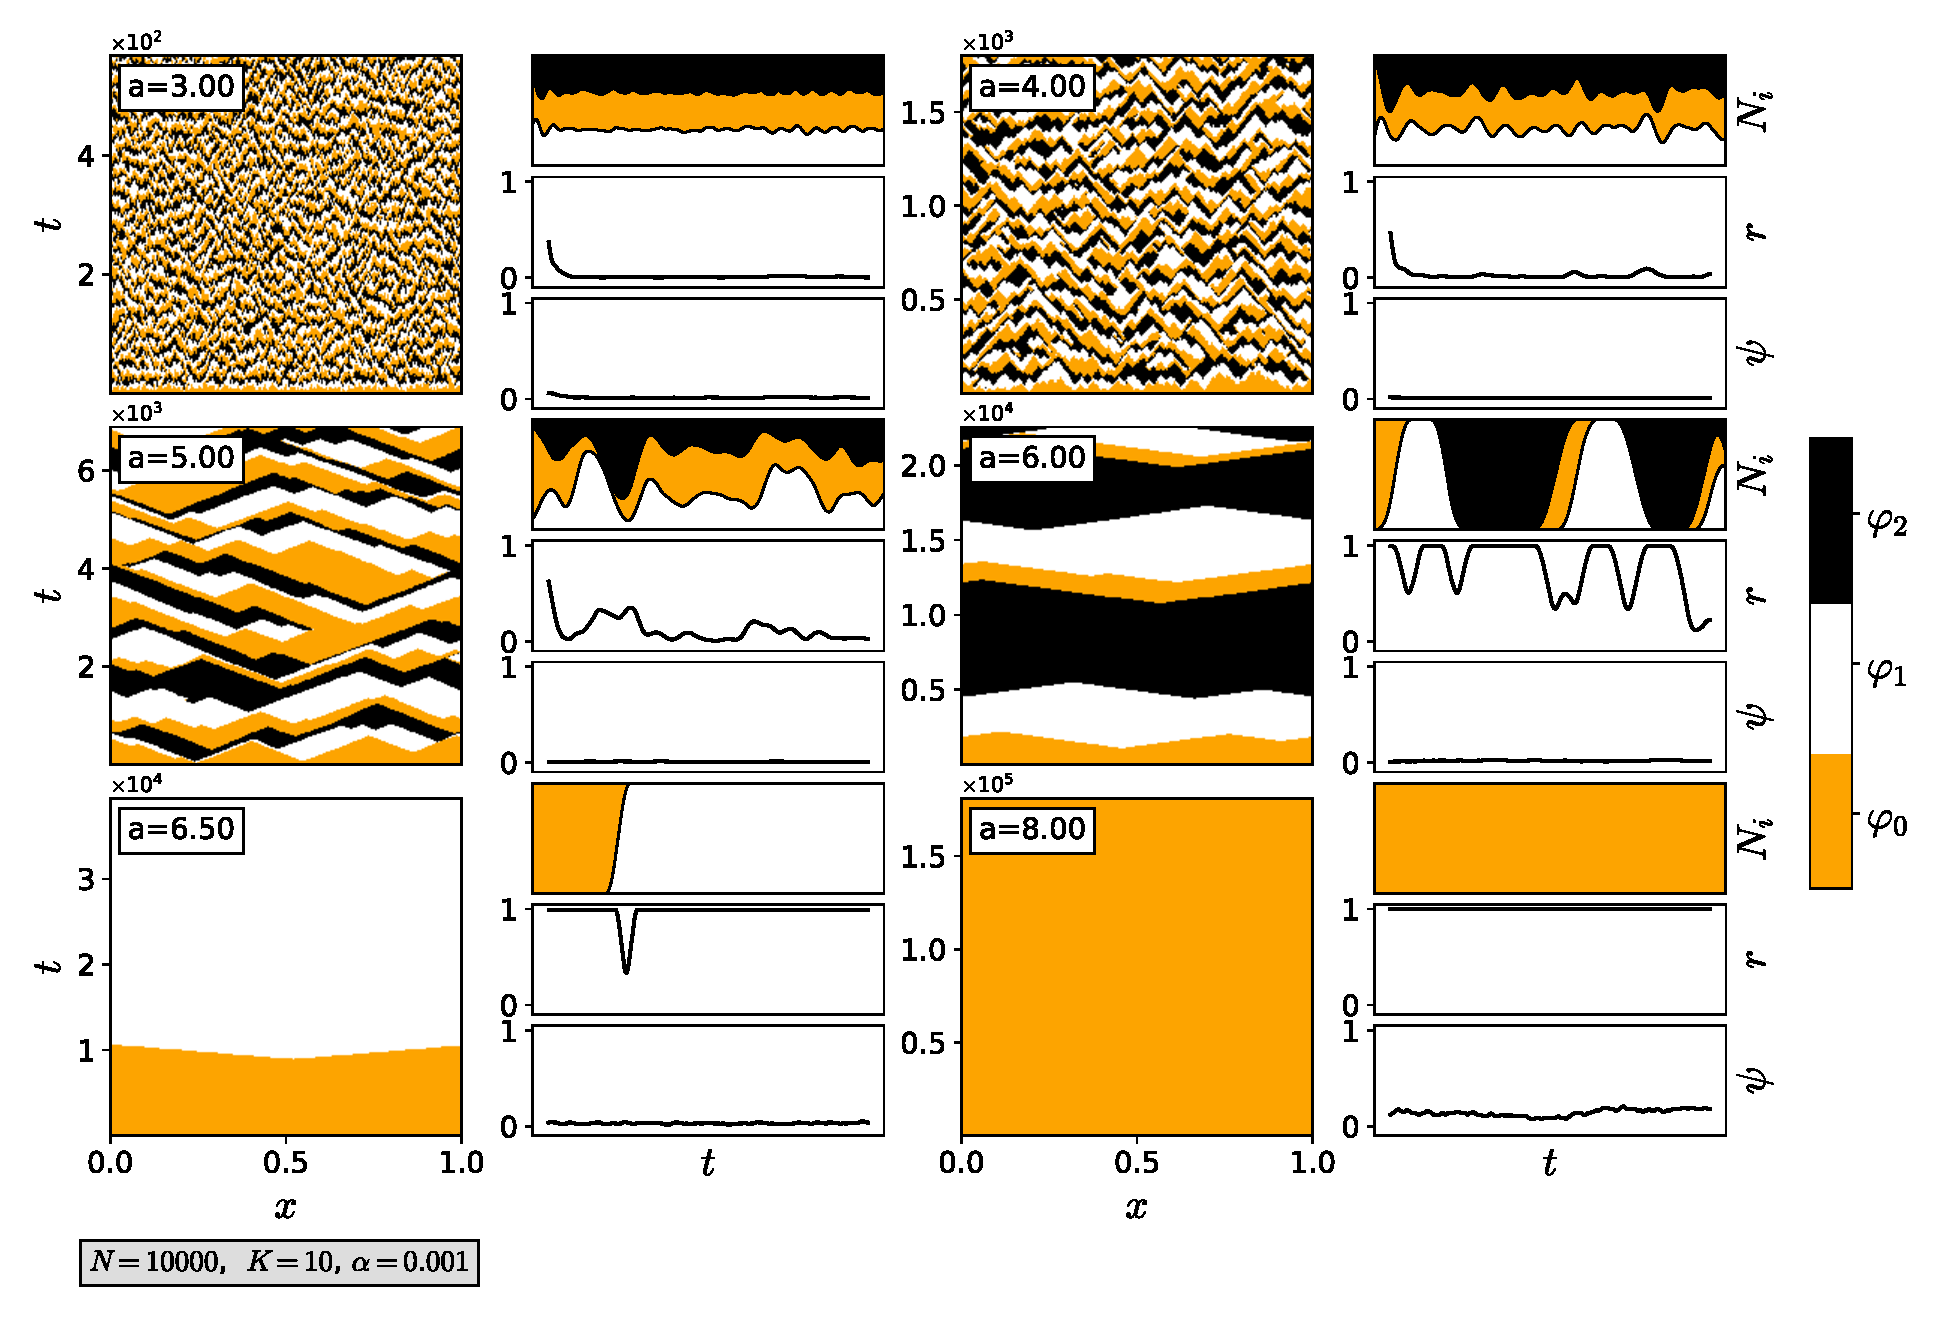
\includegraphics[width=1.\textwidth]{fig/chap2/articuno_figure_panel.eps}
\caption{\label{fig:trialpanel} Space-time plots, populations $N_i$, $\psi$ and $r$ order parameters. In all panels $N=10^4$, $K=10$
    and $\alpha=10^{-3}$. The images on the left and center-right columns show space-time plots with position on the horizontal axis
    and time increasing upward.  Adjacent and to the right of each space-time plot, three graphs show the corresponding populations,
    $\psi$, and $r$ as functions of time.  Here we see that for a large system with low connectivity there are no regular oscillations.
Instead, there are wave fronts that propagate and interfere and whose periods and amplitudes grow with $a$.  }
\end{center}
\end{figure}

Inspecting individual realizations of the dynamics in the small-$\alpha$ regime (Fig.~\ref{fig:trialpanel}) we see that the system
never shows global synchronization. It instead exhibits wave-like patterns that propagate in both directions, similar to what is
observed for large negative coupling~\cite{escaff2014arrays}, but here for $a$ positive . The amplitude and period of the wave increase
with $a$ and with system size (for fixed $\alpha$), which suggests there is an IP phase in the limit $N\to\infty$.

\subsection{Initial configuration dependence}

\begin{figure}[b]
\begin{center}
    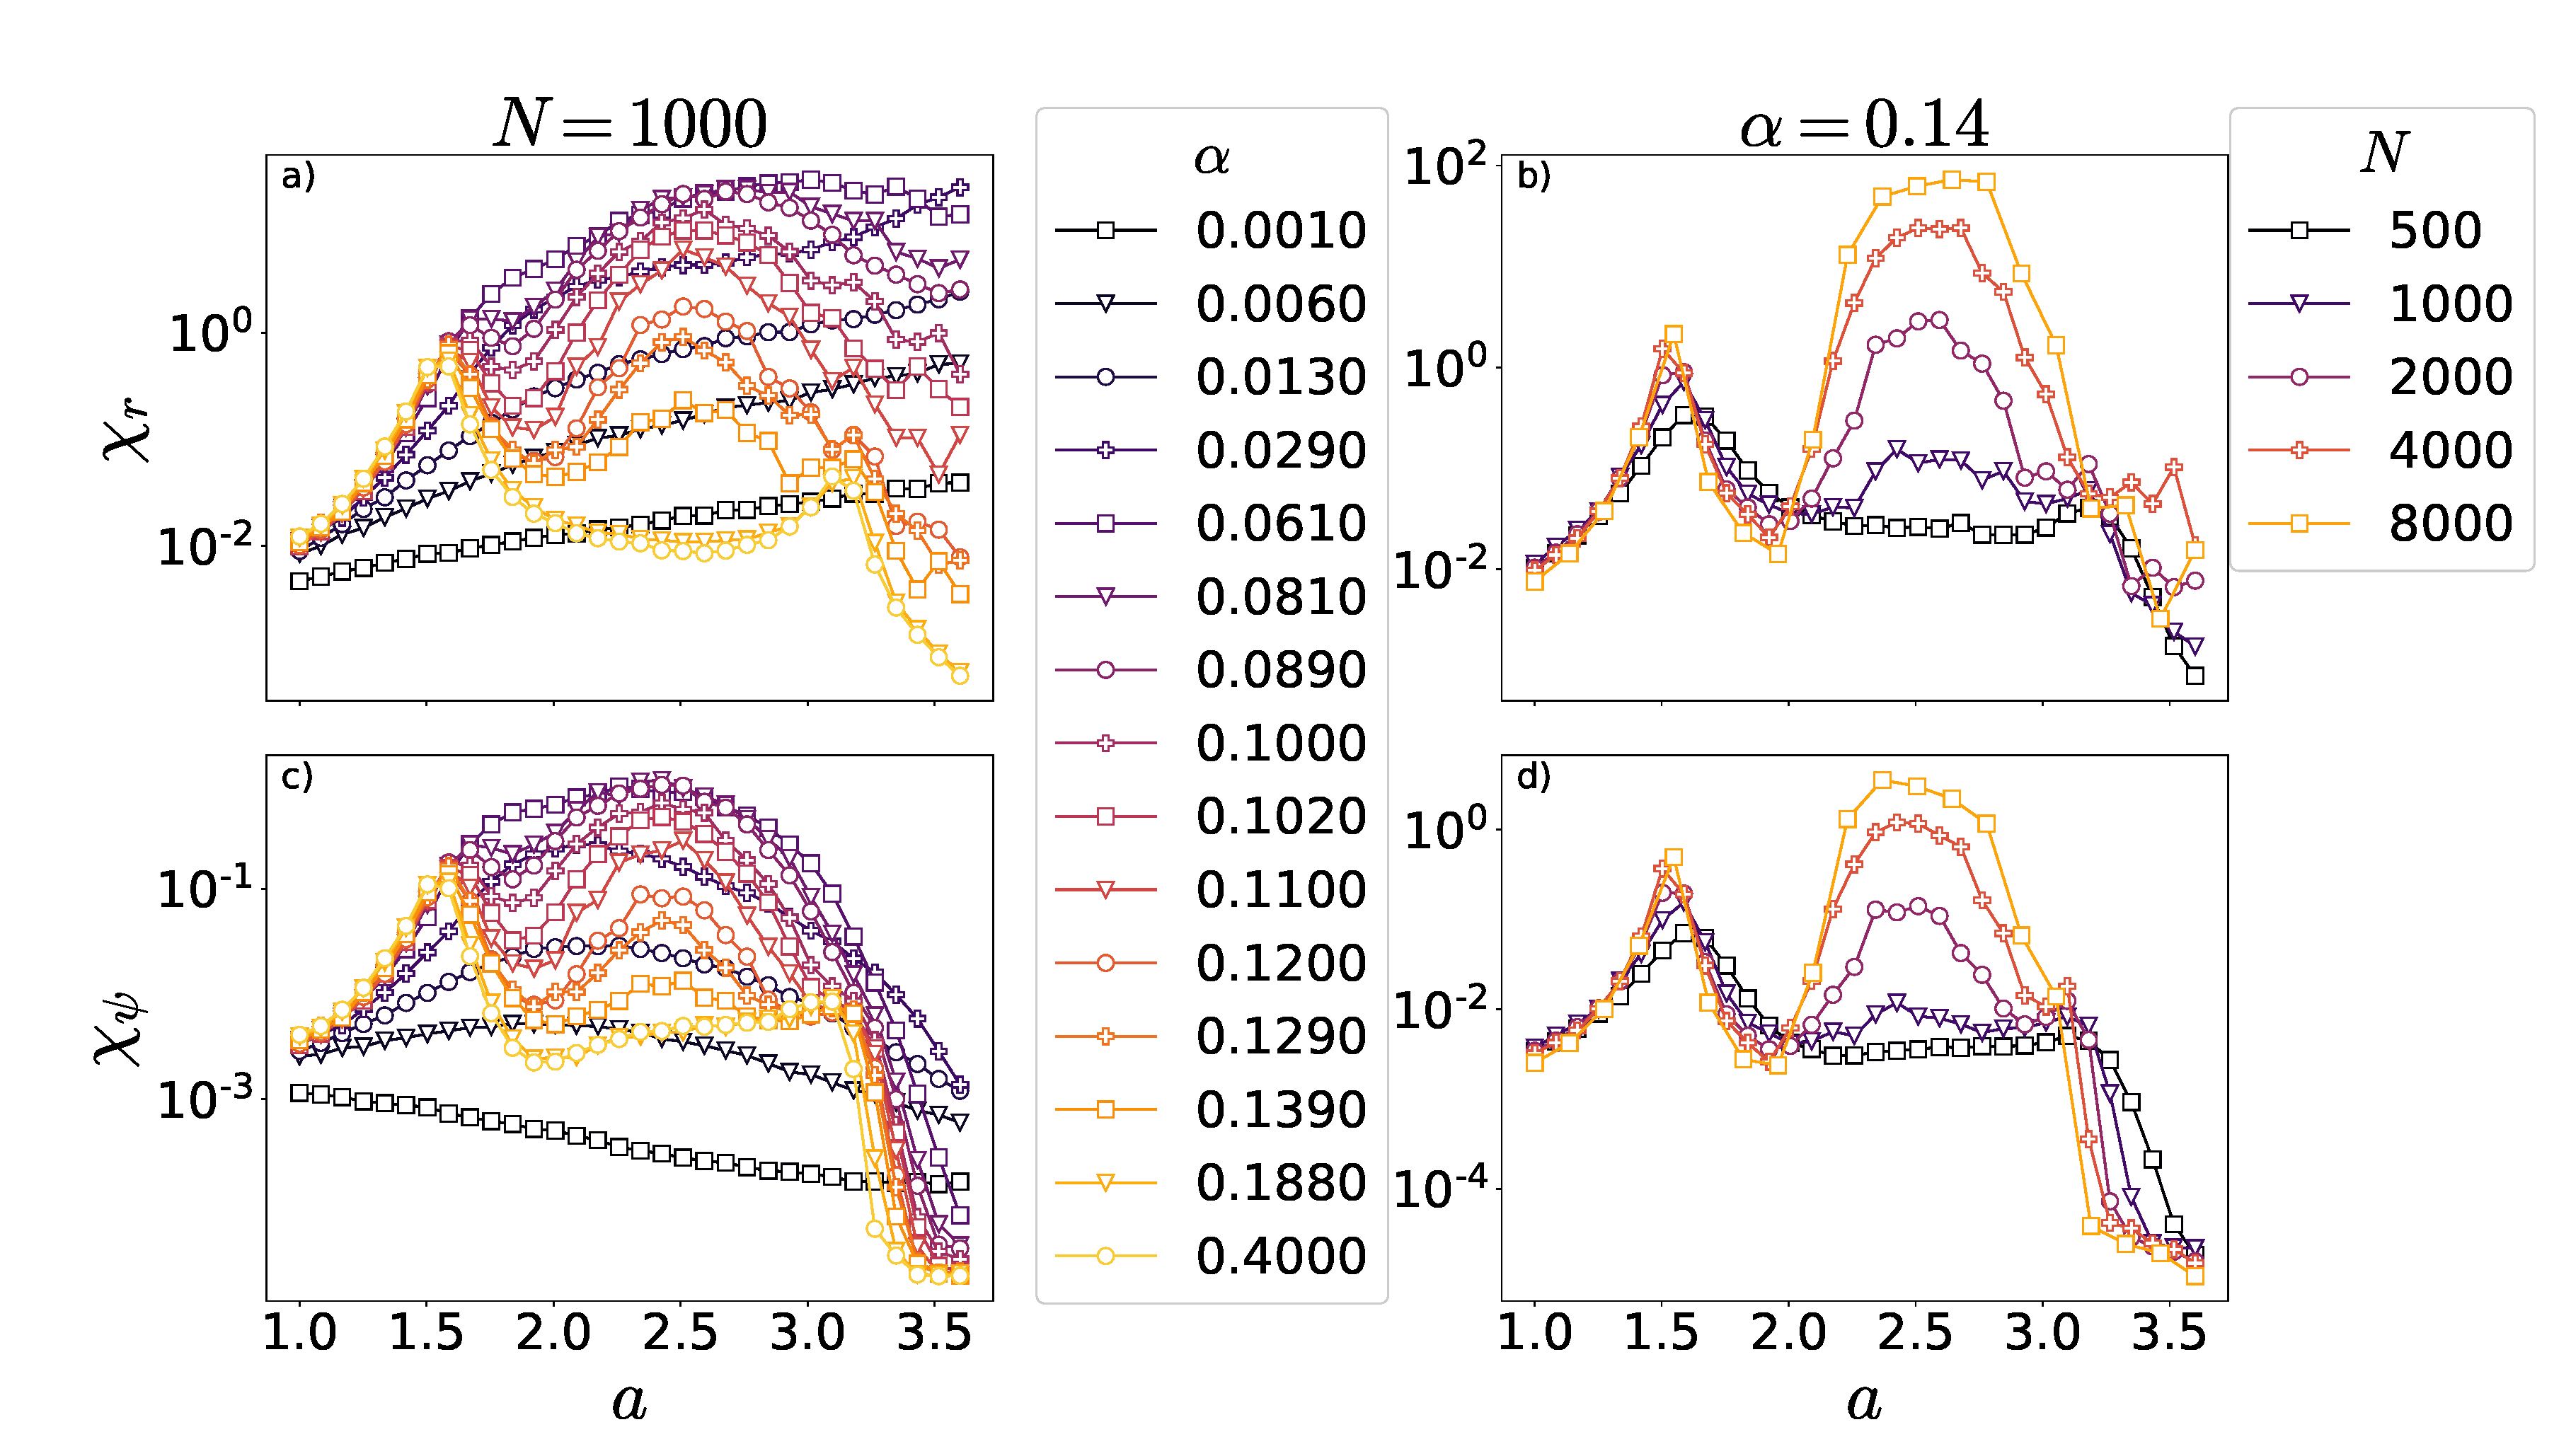
\includegraphics[width=0.95\textwidth]{fig/chap2/chi_curves_randomic.eps}
\caption{\label{fig:chicurvesrandom} (Color online) Scaled variances $\chi_r$ and $\chi_{\psi}$ for random initial conditions.  Left
column: fixed system size $N=1000$ with increasing $\alpha$.  Right column: fixed $\alpha=0.14$ and increasing system sizes.  Points
represent an average over 4000 independent realizations with random initial configurations.}
\end{center}
\end{figure}

Up to this point, all the results discussed were obtained using uniform initial configurations (ICs).  In
Fig.~\ref{fig:chicurvesrandom} shows $\chi_r$ and $\chi_{\psi}$ for \textit{random} ICs. The striking difference, compared to the results
for uniform ICs, is the presence of a middle peak between the two identified previously. The scaling behaviors (panels \textbf{b} and
\textbf{d}) suggest that the effect persists for large system sizes if $\alpha$ is held constant. High values of $\chi$ result from
multiple realizations of the dynamics that produce net averages of the order parameter that differ from one to another. At the
(continuous) GO and IP phase transitions, the values of the order parameter fluctuate strongly, giving rise to the peaks at $a=1.5$ and
$a\approx 3.1$. Another situation which may lead to high $\chi$ values is a bi-stability between configurations that have large values
of the order parameter and others having a small one, even when fluctuations associated with each configuration are small. This
suggests a \textit{discontinuous} phase transition where for some values of $\alpha$ the system can relax to multiple steady states. 

Space-time plots of the dynamics with coupling $a\approx 2.5$ and $\alpha=0.14$ reveal that this is indeed the case
(Fig.~\ref{fig:trialpanel2}).  Three examples are shown in Fig.~\ref{fig:trialpanel2}: on the left is the familiar globally
synchronized state, while the middle panel shows a travelling-wave state similar to those observed in \cite{escaff2014arrays}, (but
here, for large, positive coupling). The existence of a steady state with zero order parameter but $a>a_c$ is surprising since
Fig.~\ref{fig:chicurvesrandom} suggests that wave-like solutions persist even in the limit $N\to\infty$ (with fixed $\alpha$), where
interaction ranges become infinite.

\begin{figure}
\begin{center}
    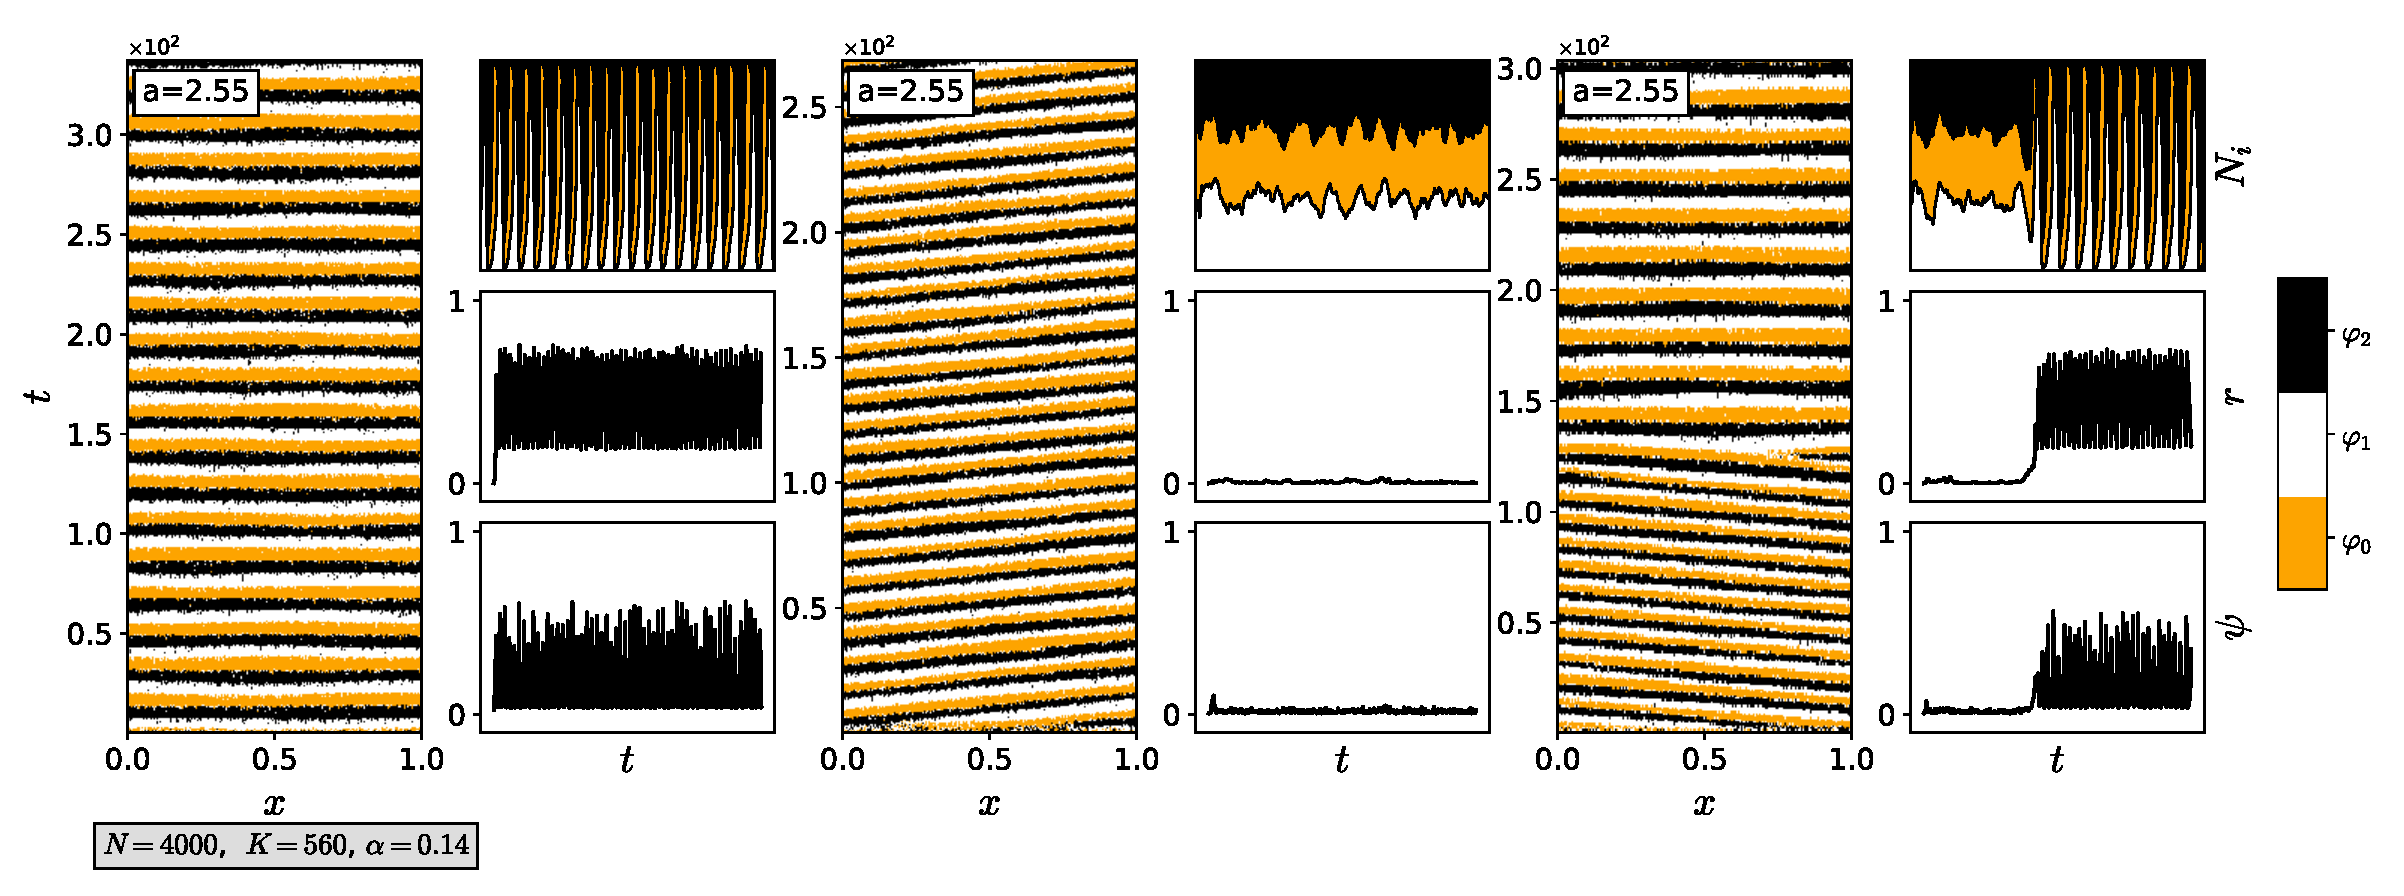
\includegraphics[width=1.\textwidth]{fig/chap2/articuno_figure_panel2.eps}
\caption{\label{fig:trialpanel2} Single realizations with random initial configurations. Left: Global oscillations. Middle: travelling
wave. Right: fluctuation-induced change from a travelling wave to global oscillations.  The fraction of realizations that converge to
travelling waves is approximately $1.6\%$. In all panels $N=4000$, $K=560$, $a=2.55$.}
\end{center}
\end{figure}

The rightmost panel in Fig.~\ref{fig:trialpanel2} shows a fluctuation-induced change from a travelling wave to global synchrony.  Such
transitions allow the average order parameter to attain values between those associated with a wave state and a globally synchronized
one, being closer to one or the other depending on what fraction of time it spent at that particular configuration.  Starting from
\textit{random} ICs, about 1.6\% of realizations exhibit travelling waves, but since $\psi\approx 0$ for the waves and $\psi \sim
\mathcal{O}(1)$ for the globally synchronized case, the variances $\chi_r$ and $\chi_{\psi}$ are sensitive even to small rates of
occurrence.  Due to fluctuations, waves do not persist in smaller systems; sizes $N \geq 700$ are required. Smaller systems exhibit
either disordered phases with domains that increase in size and duration as the coupling grows, or global synchrony if the interaction
range $K$ is large enough.  In all cases, waves with exactly one spatial period over the system are observed, while for negative
coupling, multiple stable wave numbers are found depending on the coupling magnitude \cite{escaff2014arrays}.

\begin{figure}[b]
\begin{center}
    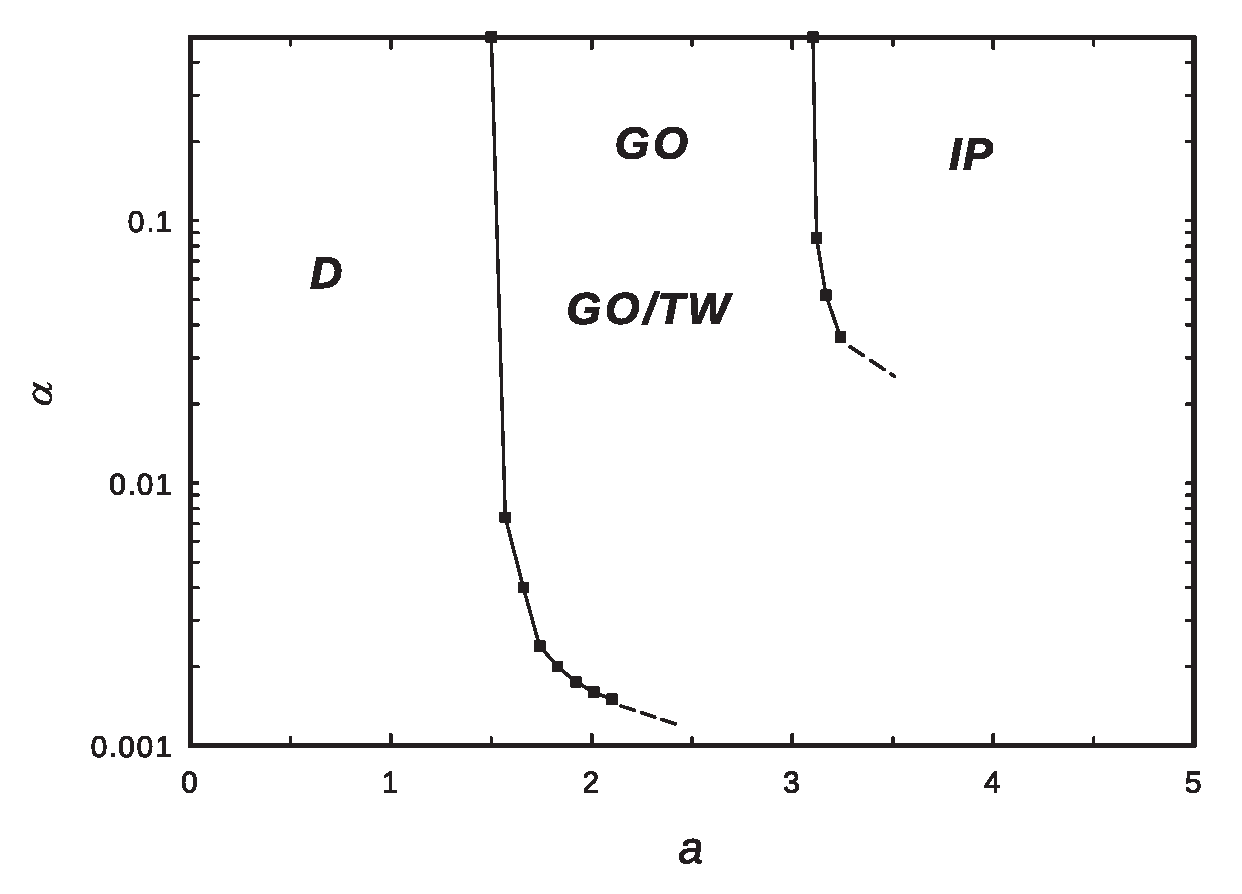
\includegraphics[width=1.\textwidth]{fig/chap2/phasediag.eps}
\caption{\label{fig:phase_diagram} Regular rings: Preliminary phase diagram in the $a$-$\alpha$ plane.  Points are simulation results
and (for $\alpha=0.5$) exact values.  Lines are guides to the eye.  Dashed lines represent our conjectures for how the phase boundaries
continue.  Phases: disordered (D); global oscillation (GO); travelling-wave (TW); infinite- period (IP).}
\end{center}
\end{figure}

The existence of travelling waves can be understood by noting that, for $\alpha<0.5$, the system consists of $G=N/2K$ domains. $G$
represents the average path length for regular rings. (See Appendix~\ref{appendix:LC}.) When $G$ is a multiple of three, the system is
capable of containing a full wavelength without oscillators in the center of the domains. The wavefronts are then able to propagate as
nucleation fronts \cite{assis2011infinite} giving rise to travelling waves. In our simulations, with $N \leq10^4$, we find only one
stable wave-number (a wave with period $N$). This is in contrast with the wave patterns observed in \cite{escaff2014arrays}, where
multiple wave-numbers were identified as stable depending on the magnitude of the coupling strength.

Although travelling waves are rare starting from random ICs, initializing with solid blocks of 0s, 1s and 2s, each occupying one third
of the system, the ensuing evolution consists of a stable travelling wave in nearly all cases.  Thus the rarity for random ICs simply
reflects the low probability of provoking a wave, and does not reflect an intrinsic instability of the travelling-wave state.  ICs with
smaller blocks, such that the system contains two or more waves, invariably yield, following a transient, a travelling wave whose
wavelength equals the system size.


With the known phase transition points for $\alpha=0.5$ and the data from Figs.~\ref{fig:chicurvesrandom} and \ref{fig:opsplit} (for $N
\leq 10^4$) we are able to sketch the phase diagram (Fig.~\ref{fig:phase_diagram}). While the phase boundaries are rather insensitive
to changes in the connectivity for relatively large $\alpha$ values, they veer to larger couplings for small $\alpha$.


\section{\label{smallworld} The WCM on small-world networks}


\begin{figure}[b]
    \centering
    \begin{minipage}[t]{0.33\textwidth}
        \centering
        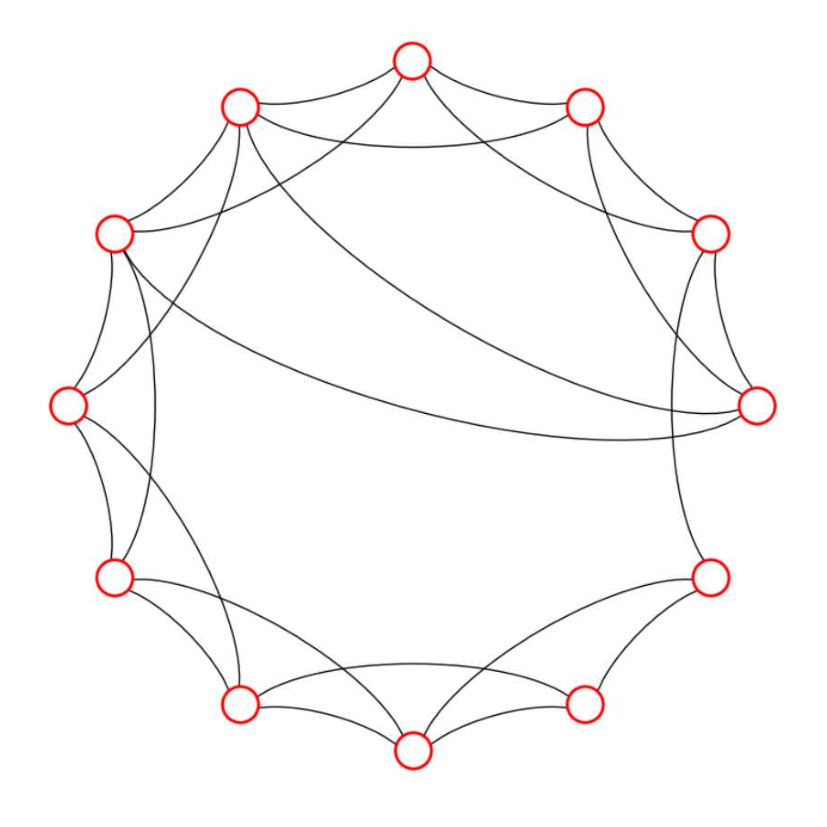
\includegraphics[width=0.9\textwidth]{fig/chap2/rewiredring.eps}
        \caption{\label{fig:rewiredring} Example of a rewired regular ring with $N=12$, $K=2$ and $p=0.1$.  }
    \end{minipage}
    \hfill
    \begin{minipage}[t]{0.62\textwidth}
        \centering
        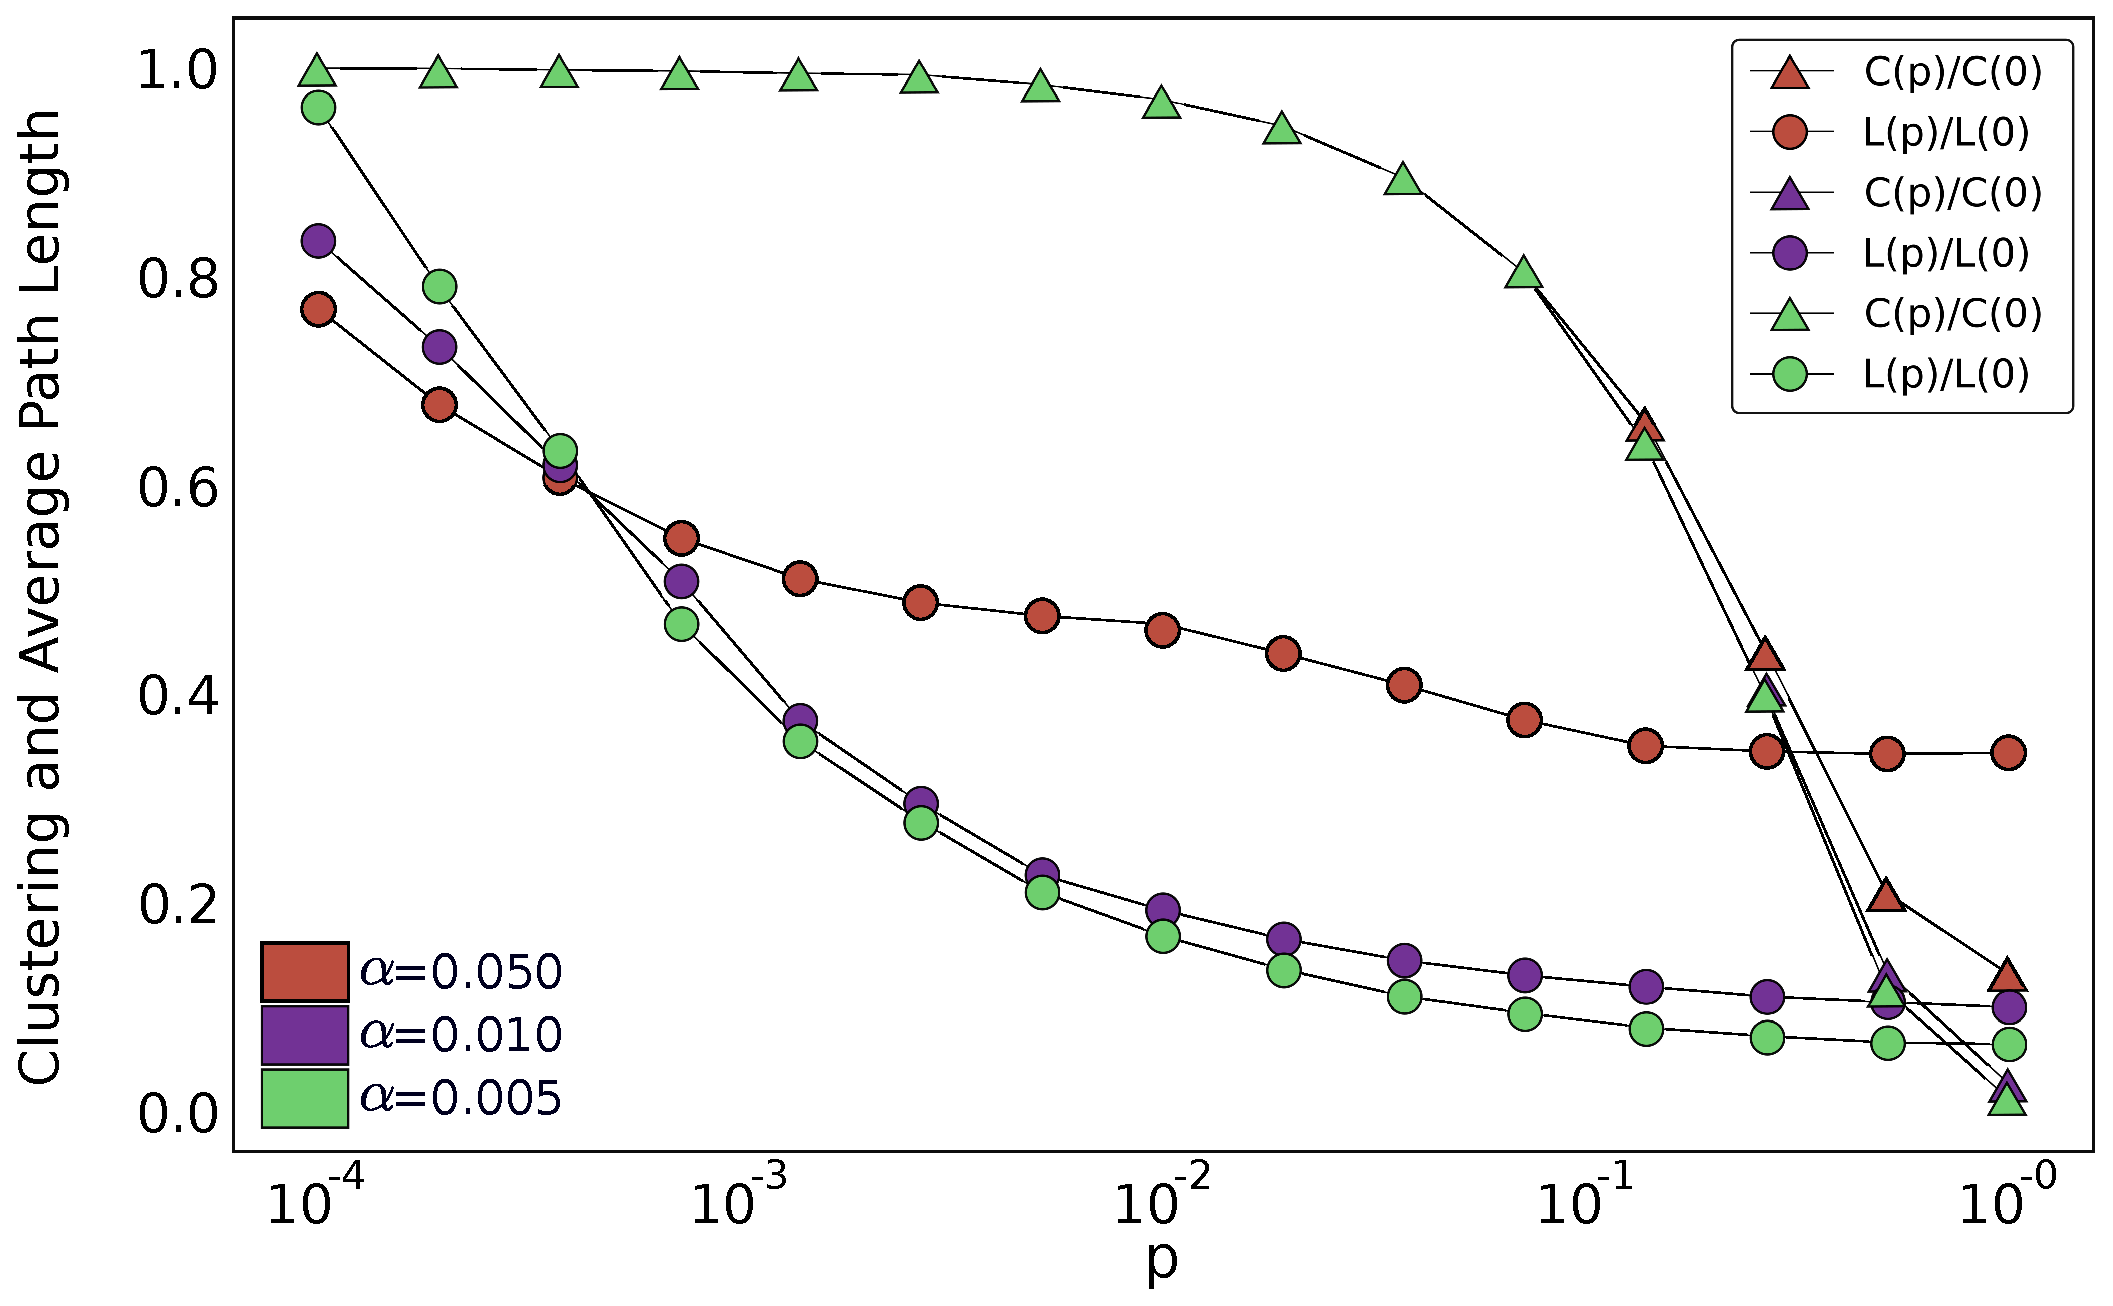
\includegraphics[width=0.9\textwidth]{fig/chap2/small-world.eps}
        \caption{\label{fig:small-world} (Color online) Clustering coefficient $C$ and mean path length $L$ versus rewiring probability
        $p$ for networks of $N=5000$ nodes.  $K=250, 50, 25$ for red, blue, green curves respectively. The data represent averages over
    400 independently generated networks.  }
    \end{minipage}
\end{figure}

Regular rings can be used as the starting point for constructing \textit{small-world networks}, which are characterized by a small degree
of separation between nodes while maintaining local regions tightly clustered. A well known algorithm for generating this type of
network from regular rings was introduced by Watts and Strogatz~\cite{watts1998collective}. Starting from a regular ring, for each edge
in the graph, the clockwise node of that edge is swapped with probability $p$ for another randomly selected node, forbidding
self-connections or repeated edges. Some care may be taken to avoid disconnected graphs as a result of this process, but this is
unlikely for most parameter triplets ($N$, $K$, $p$) considered here~\cite{watts1998collective}. An example of such a rewired ring is
shown in Fig.~\ref{fig:rewiredring}.

To characterize a network as small-world, we define two quantities:

\begin{itemize}
    \item \textit{Mean path length} $L$: For nodes $i$ and $j$ in network $\mathcal{G}$, let $L_{ij}$ be the number of edges in the
        shortest path connecting these nodes.  Then the average path length of $\mathcal{G}$ is $L=\left<L_{ij} \right>$, where the
        average is over all pairs $(i,j)$ with $i<j$.
    \item \textit{Clustering coefficient} $C$: If node $i$ has $n_i$ neighbors, then the maximum possible number of connections among
        its neighbors is $m_i=\frac{n_i(n_i-1)}{2}$. Let $m^*_i$ be the number of connections among the neighbors of node $i$ in
        network $\mathcal{G}$. Then the clustering coefficient of $\mathcal{G}$ is $C=\left< \frac{m^*_i}{m_i} \right>$, where the average is
        over all nodes $i$.
\end{itemize}

Evidently, the maximum possible value for $C$ is $C=1$ and the minimum possible value for $L$ is $L=1$. For networks generated by
rewiring a regular ring graph, $C$ and $L$ are functions of the ring-graph parameters $N$ and $K$, as well as the rewiring probability
$p$: $L\equiv L(N,K,p)$, $C\equiv C(N,K,p)$. As shown in the Appendix, for regular rings (i.e., $p=0$), we have:

\begin{equation}
C(N,K,0)=
\begin{cases}
    0 ,                                      & \text{if } K<2 \\
    \frac{3K-3}{4K-2},                       & \text{if } 2 \leq K \leq
    \frac{N-1}{3} \\
    \frac{12K^2+6K-6KN+N^2-3N+2}{4K^2-2K},   & \text{if } \frac{N-1}{3} < K <
    \frac{N}{2} \\
    1,                                       & \text{otherwise}
\end{cases}
\end{equation}

\begin{equation}
L(N,K,0)=
\begin{cases}
    \frac{KG(G-1) + rG}{N-1}, & \text{if } K \leq \frac{N}{2} \\
    1,                        & \text{otherwise},
\end{cases}
\end{equation}

\noindent where $G$ is the largest integer smaller than $\frac{N-1}{2K}$ or,
using the floor operator,

\begin{equation*}
    G = \floor*{\frac{N-1}{2K}} .
\end{equation*}

For nonzero values of $p$ we generate graphs and take the averages for $C$ and $L$, as shown in Fig.~\ref{fig:small-world}. For
rewiring probabilities $p \in \left( 0.001, 0.1 \right)$, rewiring preserves the clustering property while greatly reducing the average
path length, thus characterizing small-world networks.

\begin{figure}
\begin{center}
    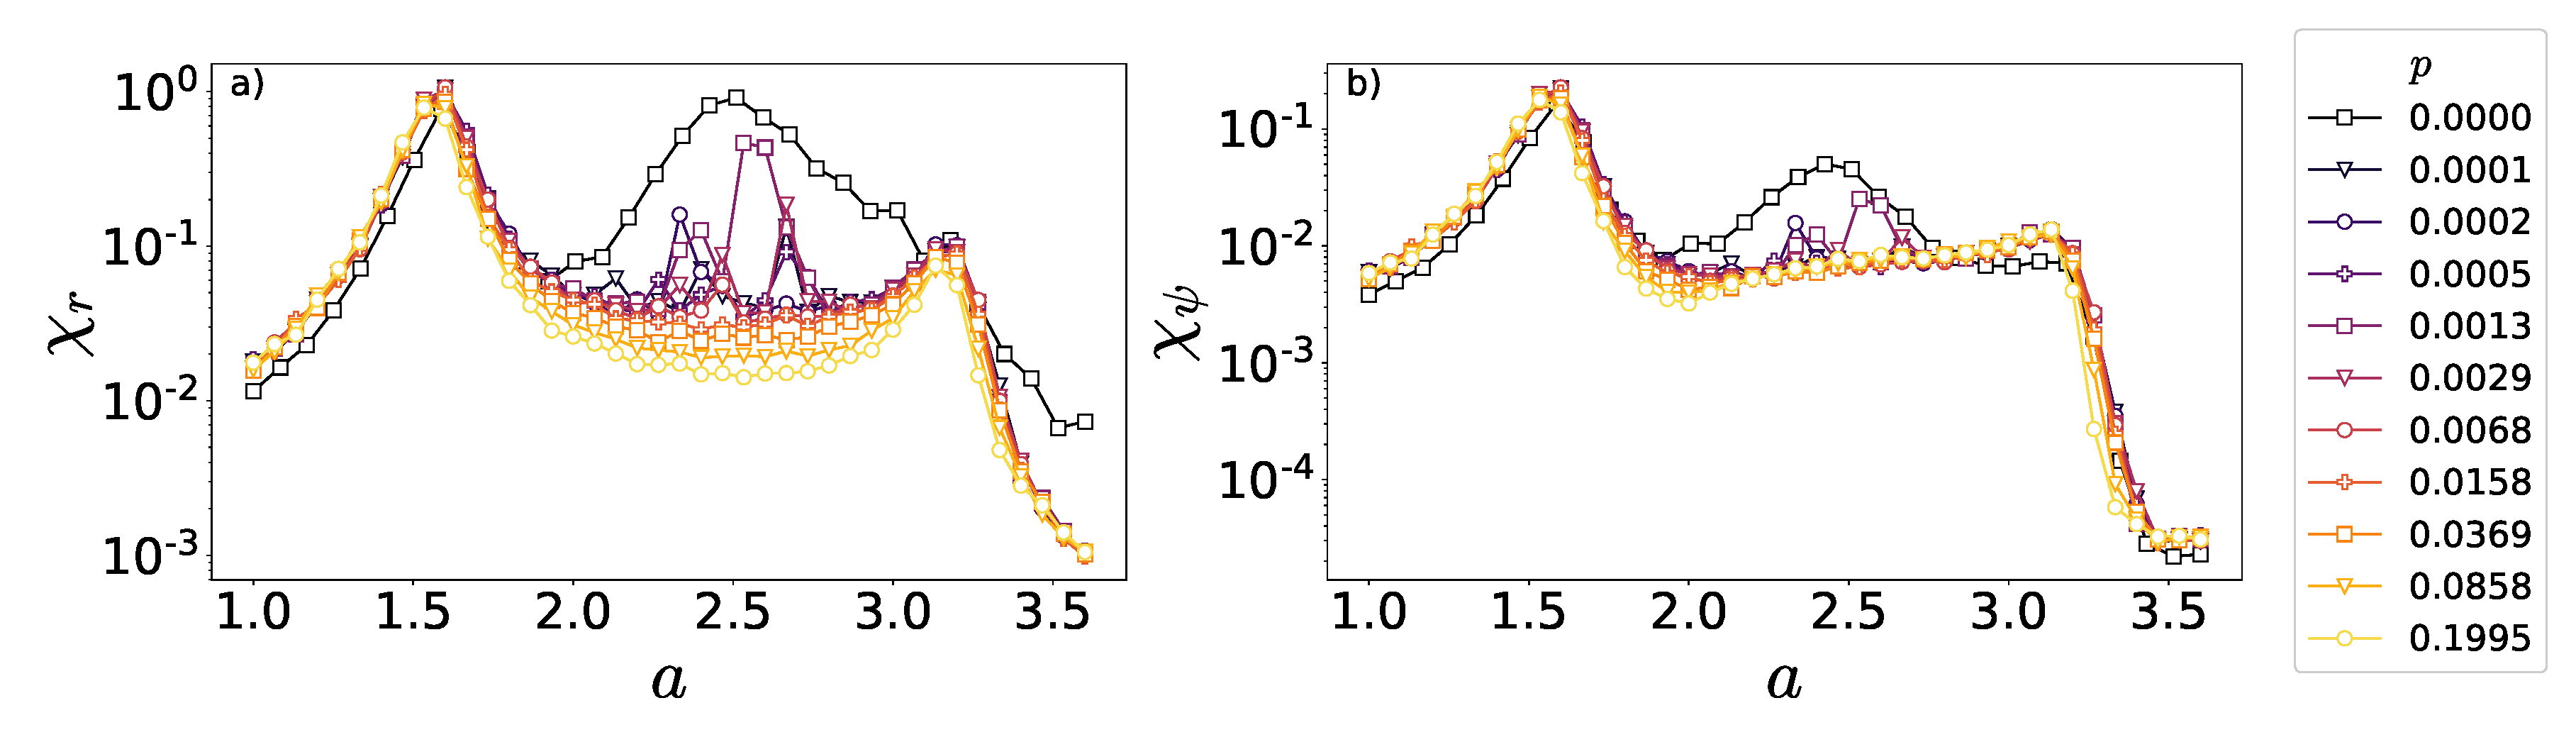
\includegraphics[width=1.\textwidth]{fig/chap2/chi_curves_pvalue.eps}
    \caption{\label{fig:chicurvespvalue} (Color online) Small-world networks: Scaled variances, $\chi_r$ and $\chi_{\psi}$, for
    increasing rewiring probabilities. $N=1000$, $K=129$, $\alpha=0.129$ with random initial conditions. For $p \approx 0.01$ the
curves follow their complete graph counterparts, even though the number of connections is half as many, and travelling waves become
unstable.  }
\end{center}
\end{figure}

\begin{figure}
\begin{center}
    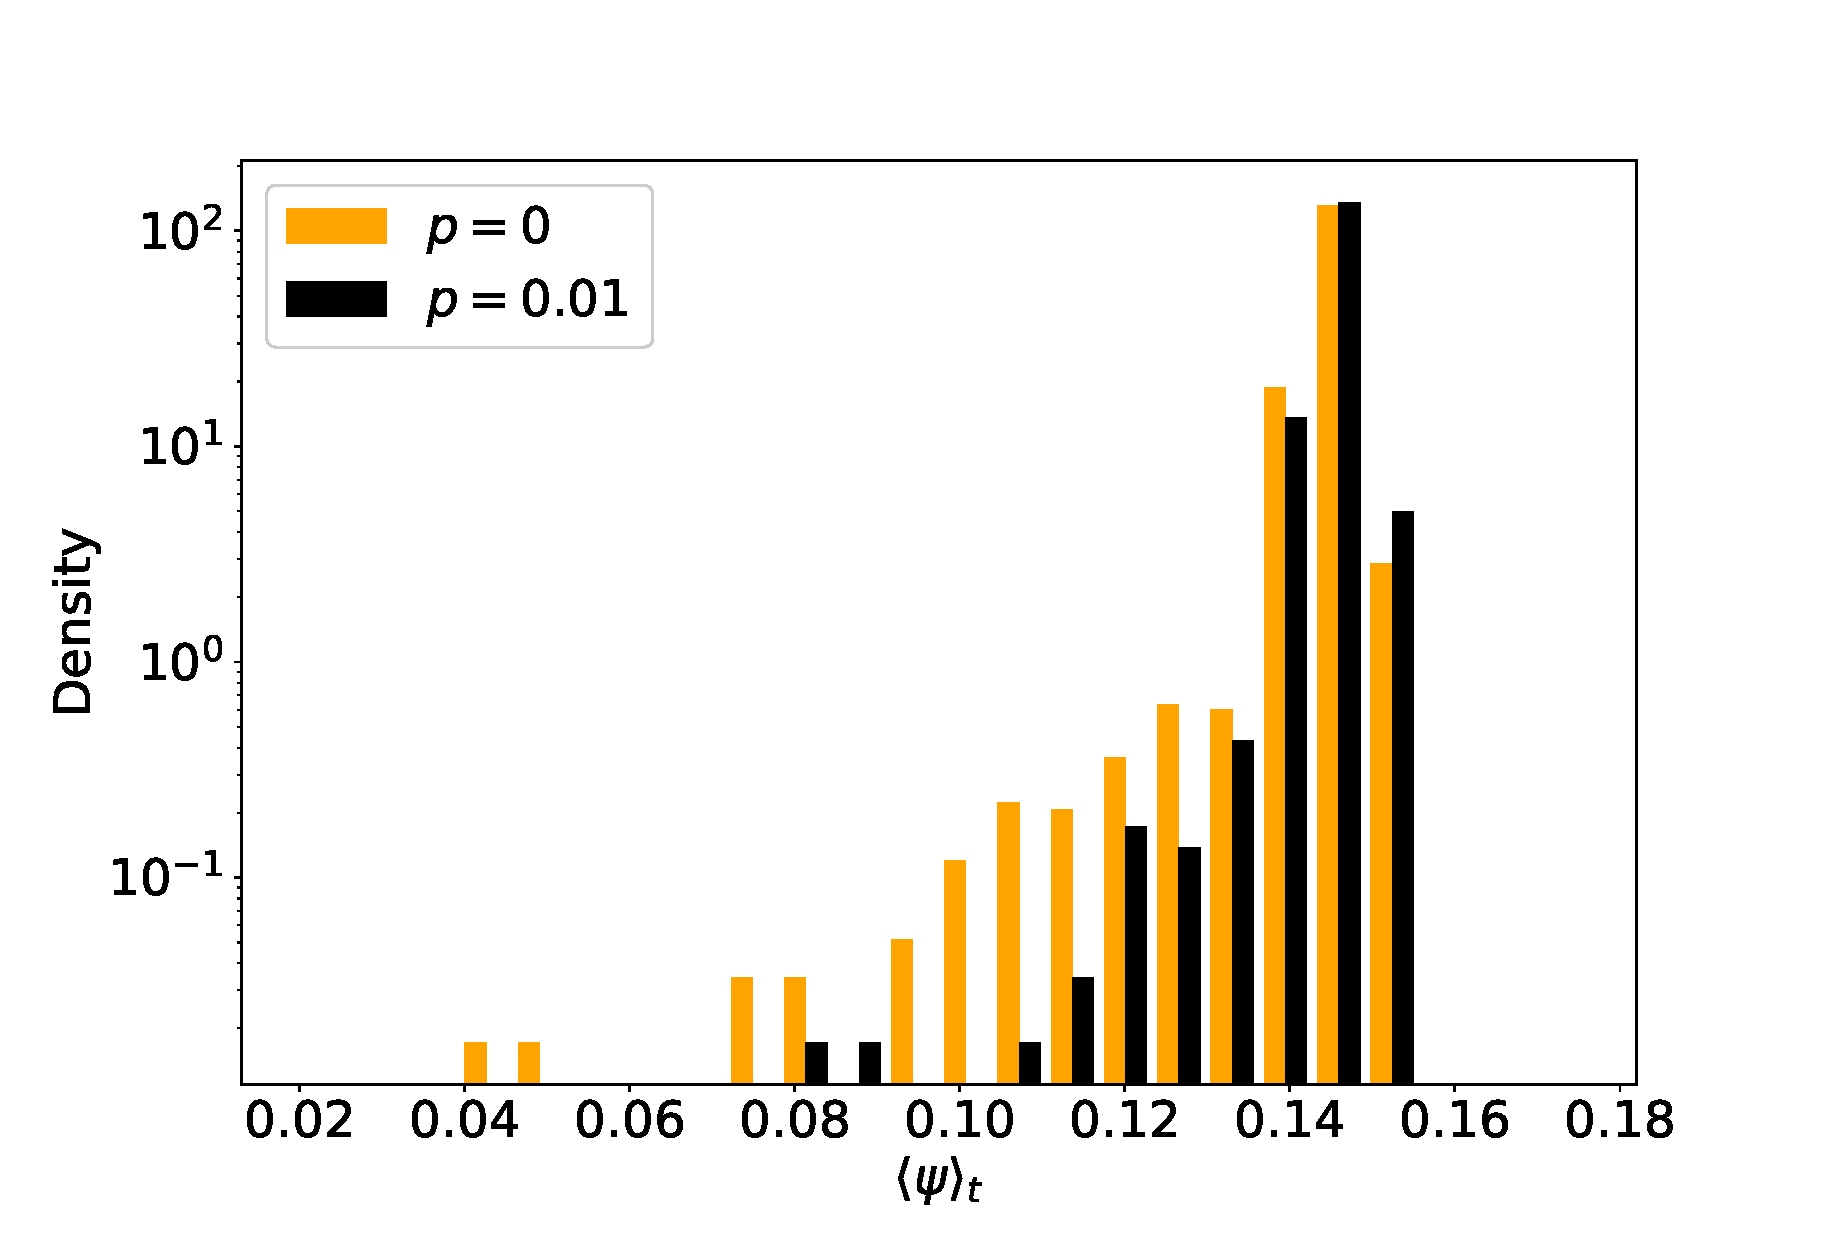
\includegraphics[width=0.8\textwidth]{fig/chap2/articuno_figure_histogram.eps}
    \caption{\label{fig:histogram} (Color online) Networks with $N=1000$, $K=129$ and coupling $a=2.5$.  Histograms of $\langle \psi
        \rangle_t$ for 9000 realizations without rewiring (yellow), and 9000 realizations with rewiring probability $p=0.01$ (black).
        The reduced frequency of small order-parameter values for $p=0.01$ compared with $p=0$ is evidence that rewiring destabilizes
        travelling waves, which are characterized by small values of $\psi$.}
\end{center}
\end{figure}

Since rewiring creates long-range interactions that reduce path lengths globally, we expect it to facilitate synchronization. This is
shown to be the case in Fig.~\ref{fig:chicurvespvalue}, where $p$ is gradually increased: realizations starting from \textit{random}
initial conditions are shown to readily synchronize for very small values of $p$, leading to the usual three phases identified for the
complete graph. This means that the introduction of very few global connections is sufficient to destabilize travelling waves; they are
virtually absent for $p \approx 0.01$. In Fig.~\ref{fig:histogram} a histogram of the average order parameter per realization, $\left<
\psi \right>_t$, shows that the fraction of time spent in wave configurations is drastically reduced by the introduction of the
rewiring procedure. When $p\geq0.01$ and $a_c<a<a^c$, the system quickly converges to the  GO phase even if it initially acquired a
wave-like solution (see Fig.~\ref{fig:trialpanel3}). Moreover, if system size is increased at constant $\alpha$, smaller values of $p$
are sufficient to cause the same effect, which is consistent with the fact that the number of long range connections is proportional to
$NK$.

\begin{figure}
\begin{center}
    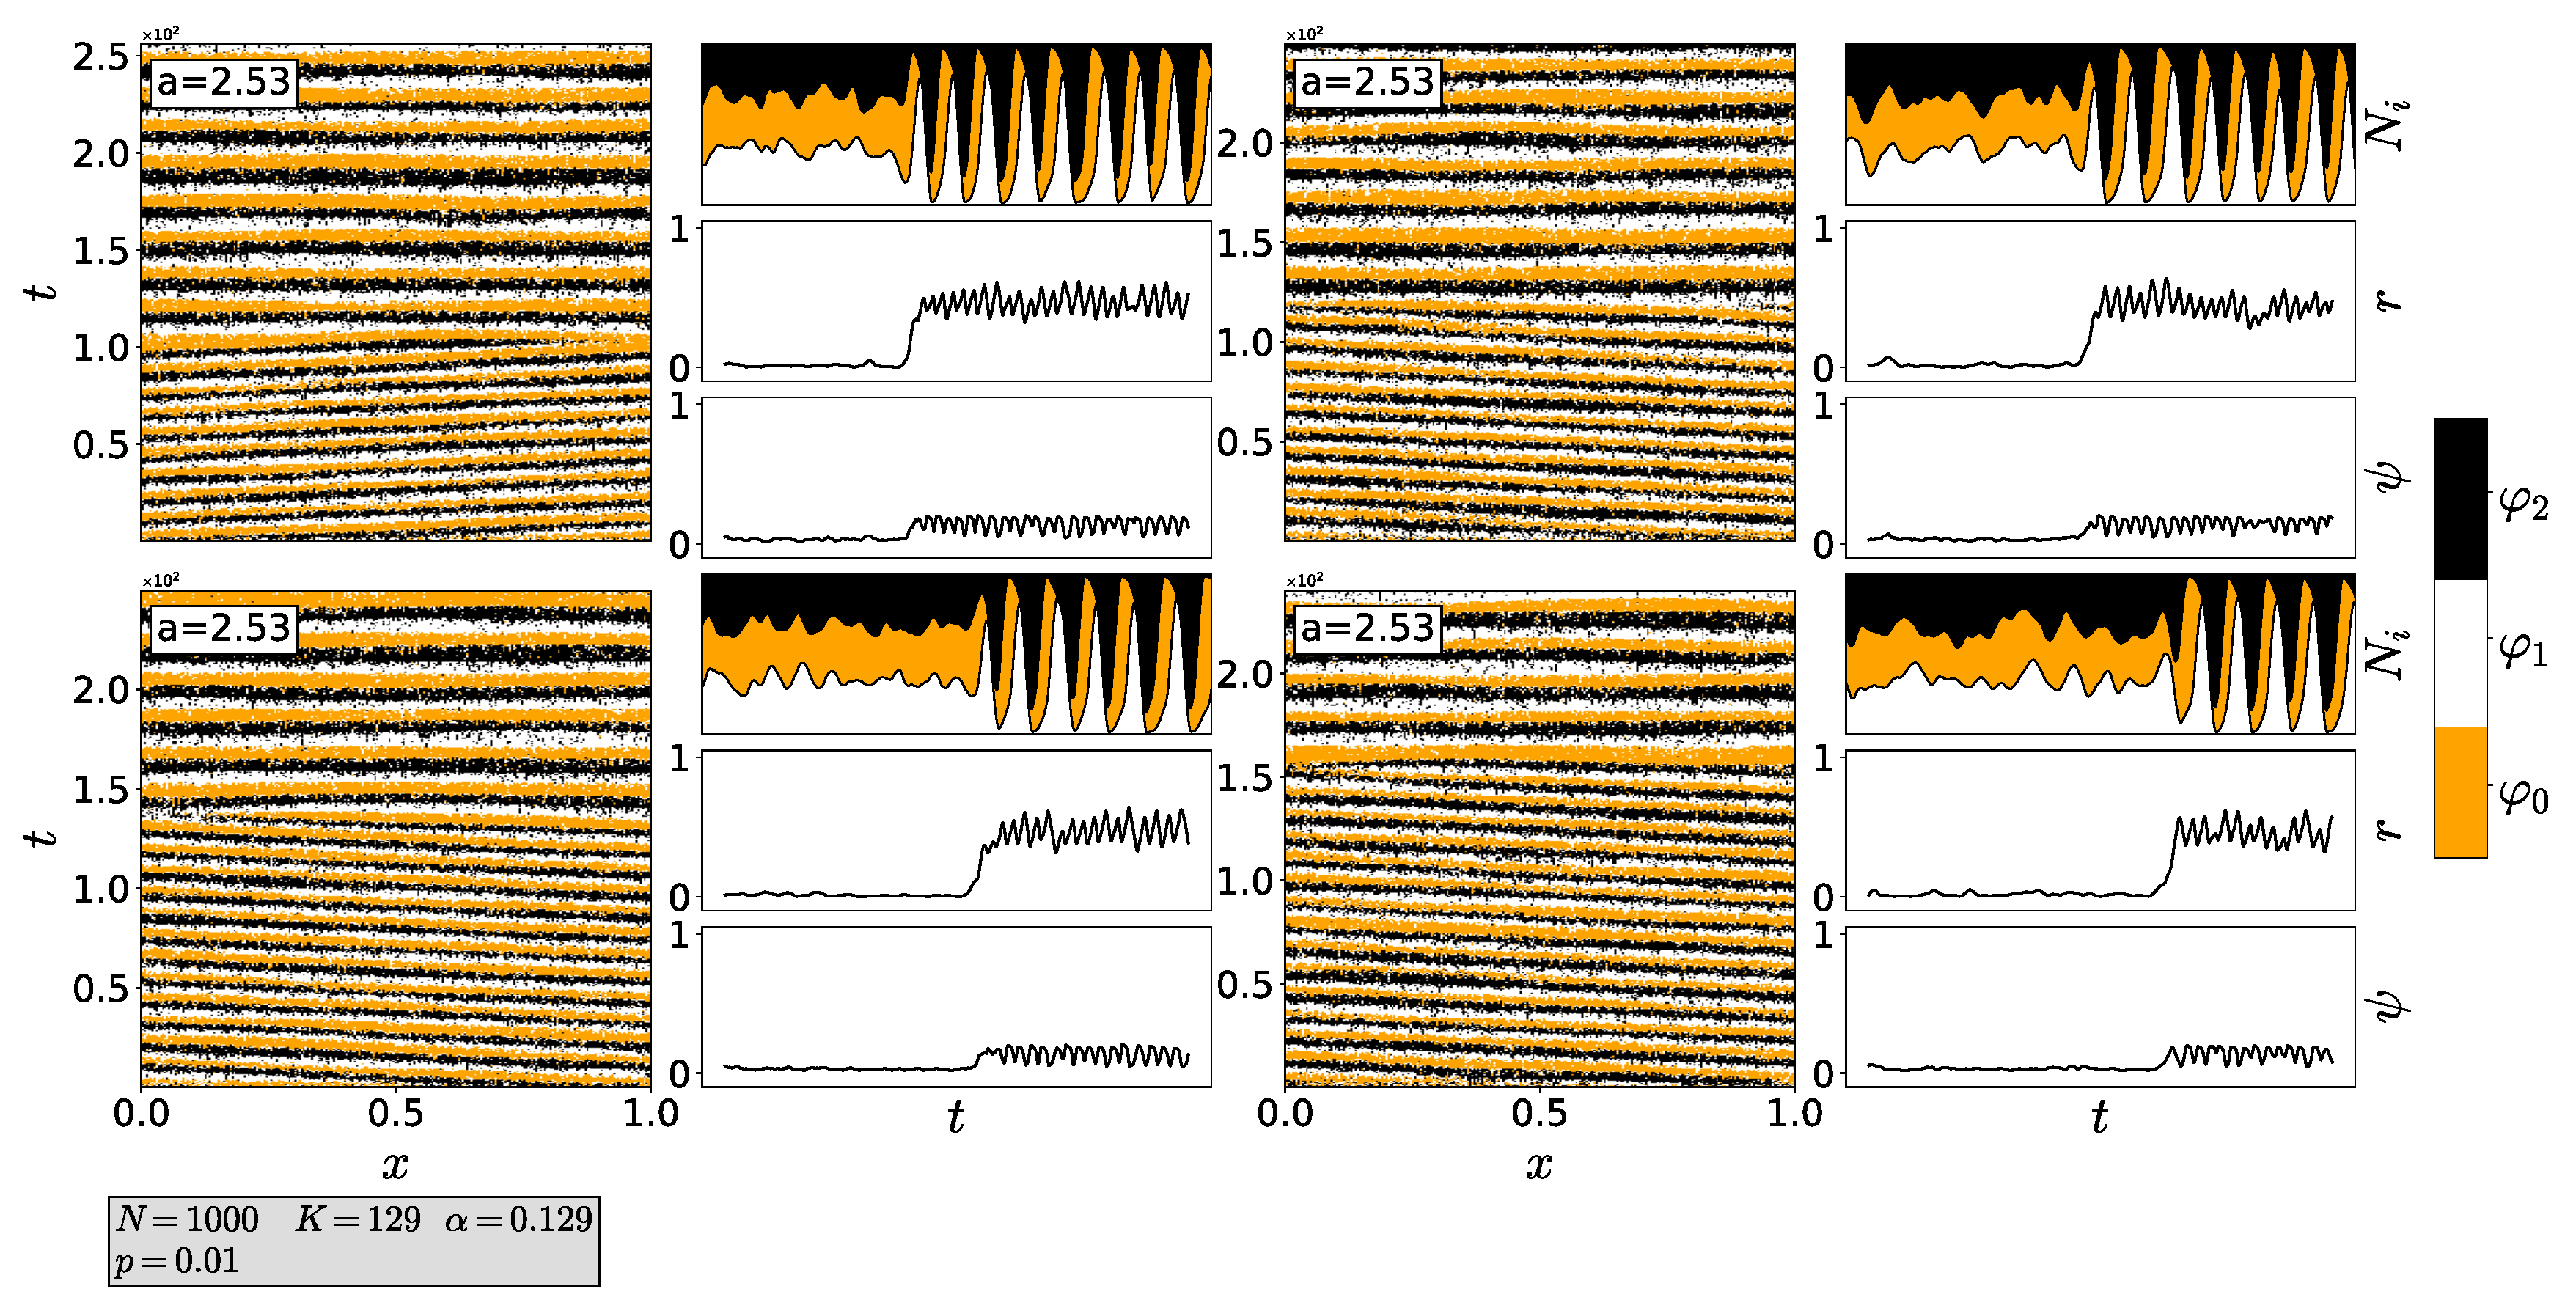
\includegraphics[width=1.0\textwidth]{fig/chap2/rewiredwavetrial.eps}
\caption{\label{fig:trialpanel3} Wave states for $N=1000$, $K=129$, $p=0.01$ and $a=2.53$. Only $0.04\%$ of realizations (measured from
9000 realizations) with \textit{random} initial configurations display traveling waves, which are also much more short-lived when compared
to the $p=0$ equivalent system.}
\end{center}
\end{figure}

Following the same procedure as before, we plot in Fig.~ \ref{fig:pvalue} the order parameters versus inverse system size $\lambda$.
Here we fix $\alpha$ at a low value ($\alpha=0.0052$) and vary $p$.  \footnote{{See full animations of figure \ref{fig:pvalue}:
\href{https://youtu.be/3iHXrDUwbqs}{GO transition}},
\href{https://youtu.be/J9OHw3DycAQ}{IP transition}}
Comparing these results with panels d) and h) of Fig.~\ref{fig:opsplit} we see that the mean absolute value of $\psi$ is much greater
when $p$ lies in the small-world region, indicating greater synchrony among oscillators. Space-time plots for values of $p>0$ show that
indeed travelling waves become unstable, so that the system exhibits only the three phases observed on the complete graph, namely,
disordered, GO and IP phases. The phase diagram remains similar to the case of regular rings, displaying low sensibility to $\alpha$
except for very small values where the discreteness of finite systems becomes apparent. The main difference is that for any positive
$p$ wave-like steady states are absent and thus the phase diagram contains only three macroscopically distinct phases.

\begin{figure}
\begin{center}
    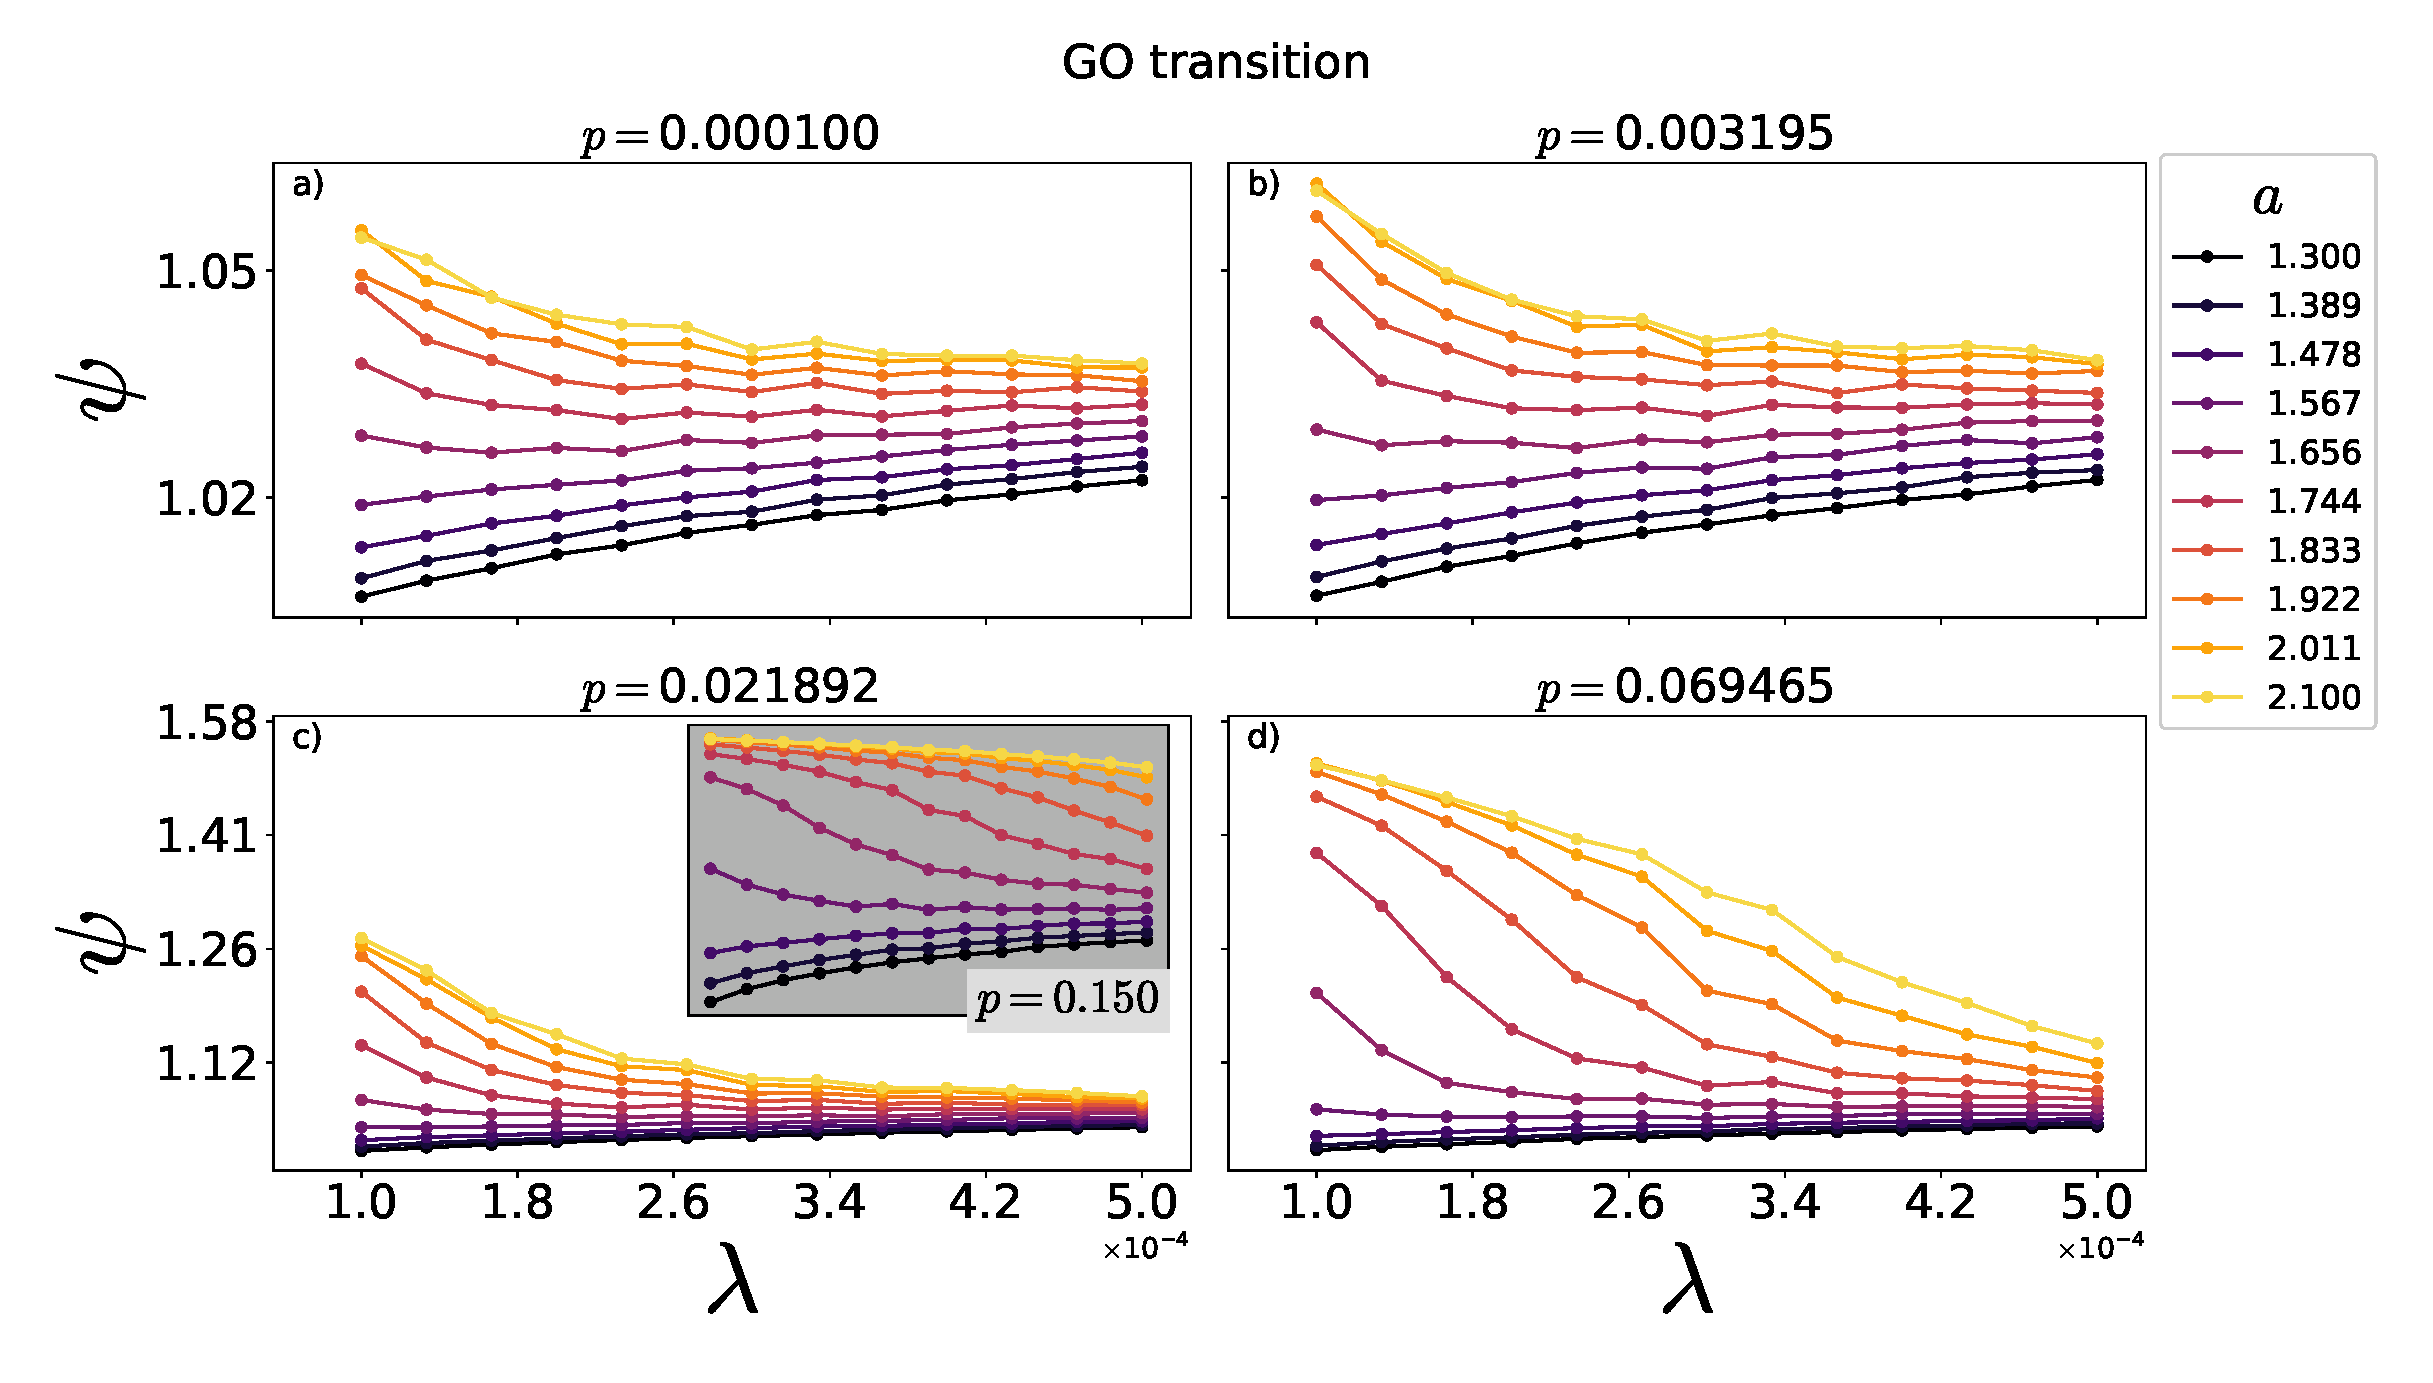
\includegraphics[width=0.9\textwidth]{fig/chap2/opsplit-psi-GOT-pvalue.eps}
    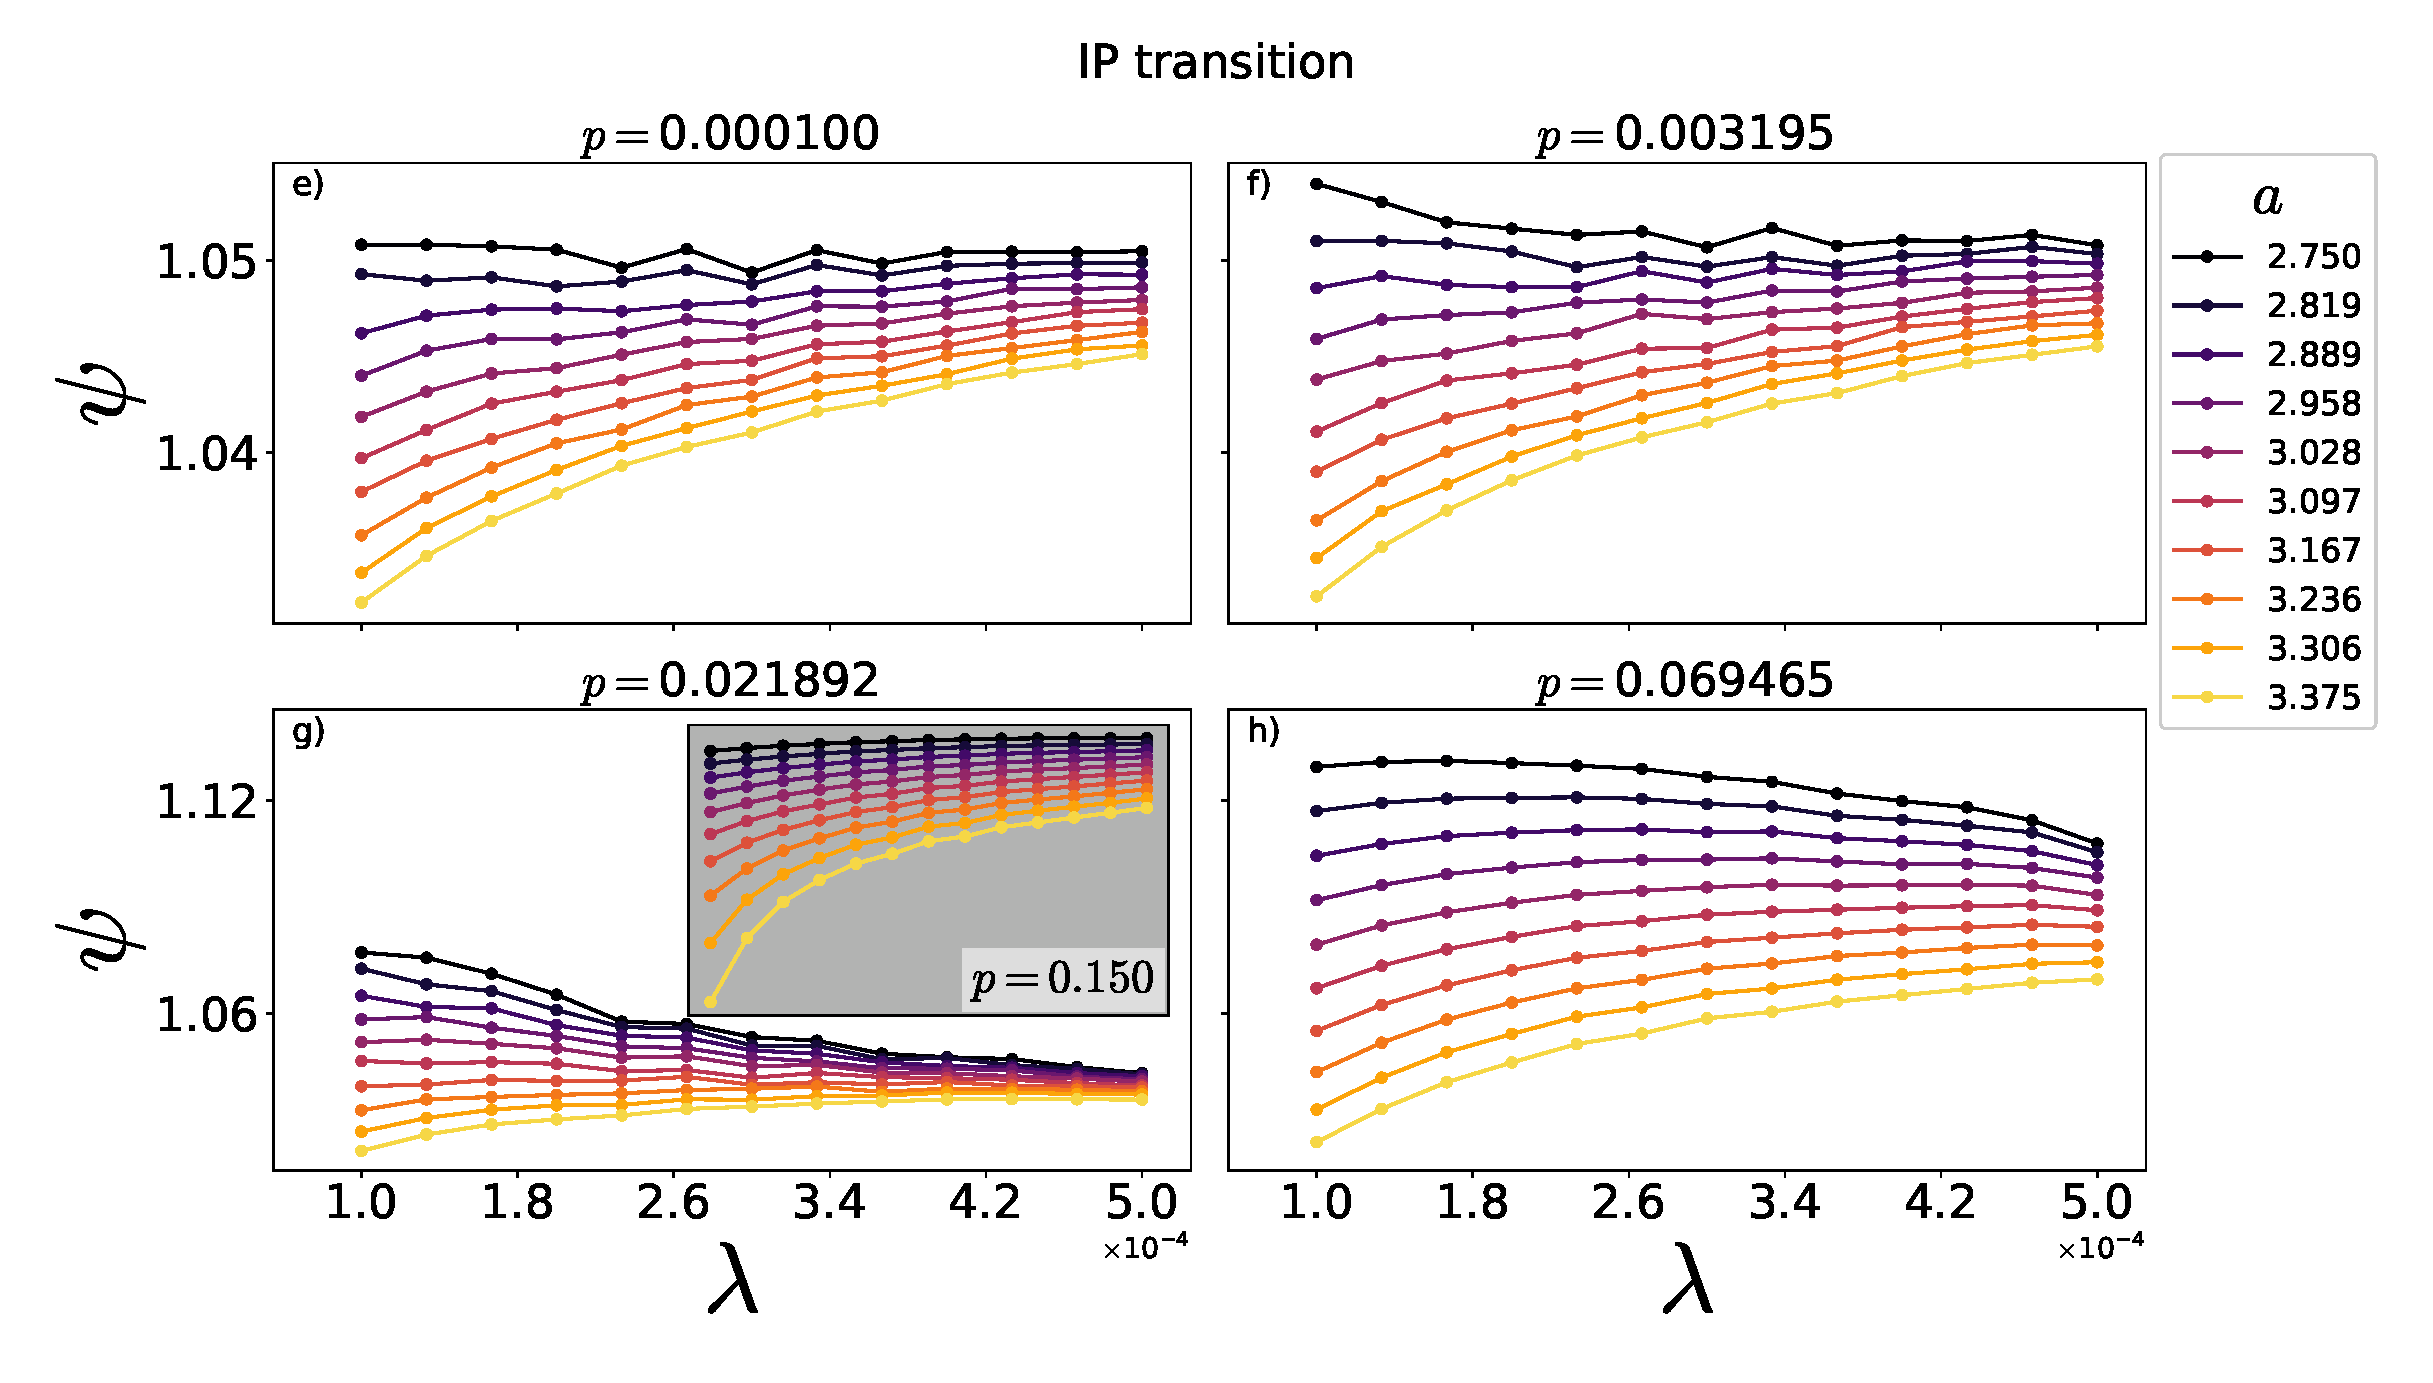
\includegraphics[width=0.9\textwidth]{fig/chap2/opsplit-psi-IPT-pvalue.eps}
\caption{\label{fig:pvalue} (Color online) Order parameter $\psi$ versus inverse system size $\lambda$ for $\alpha=0.00524$ and various
values of rewiring probability $p$ and couplings around the GO and IP transitions. Insets show the behavior for $p=0.15$, the highest
rewiring probability used.}
\end{center}
\end{figure}

\clearpage


\section{\label{conclusions}Conclusions}


We study the WCM model, a discrete-phase oscillator model exhibiting global synchronization and an infinite-period phase, on regular
ring lattices and small-world networks.  Each oscillator is coupled to a nonzero fraction $\alpha$ of the others, but the connectivity
is in generally much smaller than for a complete graph.  Our results support the conjecture that all three phases - disordered,
globally synchronized, and infinite-period - appear for any nonzero connectivity $\alpha$. 

Surprisingly, travelling waves also appear in the small-$\alpha$ regime on regular ring lattices;  such waves may represent a
long-lived metastable state.  (A previous study identified waves in the anti-coupling case \cite{escaff2014arrays}.) In our studies
travelling waves constitute only about $1.6\%$ of the steady states reached from starting from \textit{random} initial configurations,
and are prone to decay into global oscillations due to fluctuations when system size is small.  The introduction of long-range
interactions through rewiring (i.e., using the Watts-Strogatz algorithm) can lead to synchronization without increasing the total
number of connections.  Rewiring also suppresses travelling waves by introducing long range interactions.

The fact that regular rings are capable of sustaining travelling waves for $a>a_c$ is surprising, showing that networks of oscillators
might fail to synchronize even in the presence of nonlocal interactions and strong coupling, conditions which are sufficient for the
synchronization on hypercubic lattices of dimensions greater than 2 as well as on the complete graph. This raises the possibility that
WMCs admit wave-like steady states on cubic lattices, similar to oscillations observed in the two-dimensional Belousov–Zhabotinsky
reaction.

Several other questions remain open for future study, for example, whether travelling waves represent a stable phase for some range of
parameters, or are always metastable, and whether waves of wavelength smaller than the system size $N$ are possible.  We have sketched
a phase diagram for ring lattices, but detailed information for the small-connectivity regime is lacking.  Since the model exhibits a
pair of continuous phase transitions, it is of interest to develop a full scaling picture, including the effect of ordering fields
conjugate to the order parameters.  Finally the question of what simple external  perturbations are capable of destroying
synchronization or the symmetry-broken phase may be of some practical interest.

